\documentclass[12pt,oneside,a4paper]{article}

%% Language and font encodings
\usepackage{textcomp}
\usepackage{ulem}
\usepackage[danish,english]{babel}
\usepackage[utf8x]{inputenc}
\usepackage[T1]{fontenc}

%% Sets page size and margins
\usepackage[left=2.5cm,top=2.0cm,bottom=1.5cm, right=3.0cm]{geometry}

%% Useful packages
\usepackage{amsmath}
\usepackage{graphicx}
\usepackage{epsfig}
\usepackage[colorinlistoftodos]{todonotes}
\usepackage[colorlinks=true, allcolors=blue]{hyperref}
\usepackage{gensymb}
\usepackage{float}
\usepackage{adjustbox}
\usepackage{graphics}
\usepackage{amssymb}
\usepackage{url}
\usepackage{cancel}
\usepackage{booktabs}
\usepackage{pdfpages}
\usepackage{mathpazo}
\usepackage[section]{placeins}
\usepackage{caption}
\usepackage{wrapfig}
\usepackage{tocloft}
\usepackage{subfig}
\usepackage{fancyhdr}
\usepackage{framed}
\usepackage{footnote}
 \usepackage{url}

\linespread{1.3} % linjeafstand 1.5
\setlength{\parindent}{0cm}
\setlength{\parskip}{0.3cm}

\begin{document}
\selectlanguage{danish}
\pagenumbering{roman}

%% Forside %%

\begin{center}
    {\textsc {\LARGE \bf{Københavns Universitet \\[0.3cm]  Bachelorstudiet i fysik}}}\\[1.5cm]
    {\textsc {\Large \bf Førsteårsprojekt 2017}}\\[0.8cm]
    {\Large Projekt nummer: 2017-05}\\[1cm]
    
    \rule{15cm}{0.01cm}\\[1cm]
    {\LARGE\bf  Simulering af neutron optik} \\ {\it Med fokus på optimering af spejlkvalitet}\\ [0.5cm]
    \rule{15cm}{0.01cm}\\[1cm]
\end{center}

\vfill
{\large Forfattere:}\\
{\large \hspace*{1cm} \makebox[6cm][l]{Jonas Peter Hyatt}  \hspace{1cm} KU- ID: \makebox[2cm][l]{ZKV499} \\
{\large \hspace*{1cm} \makebox[6cm][l]{Waldemar Svejstrup}   \hspace{1cm} KU- ID: \makebox[2cm][l]{MDS274} \\
{\large \hspace*{1cm} \makebox[6cm][l]{Jens Walter Birkemose}   \hspace{1cm} KU- ID: \makebox[2cm][l]{SMX359} \\ 
        
{\large Vejledere:}\\
{\large \hspace*{1cm} \makebox[6cm][l]{Kim Lefmann}  \hspace{1cm} Email: \makebox[2cm][l]{lefmann@nbi.ku.dk} \\
{\large \hspace*{1cm} \makebox[6cm][l]{Jonas Okkels Birk}    \hspace{1cm} Email: \makebox[2cm][l]{jonasobirk@gmail.com} \\

\vfill

{\large Rapporten omfatter {\bf 1} siders hovedtekst og {\bf 1} siders appendix.}

{\large Rapporten er indsendt som en pdf-fil den 17 marts 2017. }

\normalsize

%% Forside slut! %%
\newpage
%% Abstract %%

\begin{abstract}


Dansk:
\\
Vi har arbejdet med neutronoptik, der skal anvendes ved ESS i Sverige. Her har vi nærmere betegnet arbejdet med guidesystemerne, der transporterer neutronerne, fra neutronkilden, til den prøve der ønskes undersøgt. Her har vi gjort brug af simuleringsprogrammet McStas, der bruger Monte Carlo simuleringer, til at simulere neutronernes vej gennem diverse guides. Her har vi arbejdet med flere forskellige guides, og til slut optimeret på en guide, der måske bliver bygget ved ESS. \\

Engelsk:
\\
We have worked on neutronoptics at ESS in Sweden. Here we have worked with the guidancesystems that transport the neutron from the neutronsoruce, to the sample that are going to be 
\end{abstract}

%% Abstract slut! %%
\newpage
%% Indholdsfortegnelse %%

\tableofcontents

%% Indholdsfortegnelse slut %%
\newpage
%% Rapporten begynder her! %%

\pagenumbering{arabic}

\section{Introduktion}

Vores samfund har, over de sidste par hundrede år, været under en rivende udvikling. Mange nye opfindelser er blevet skabt, og mange gamle opfindelser er blevet optimeret. I vores søgen efter mere, leder vi konstant efter nye og bedre måder at gøre tingene på. På trods af den teknologiske udvikling, har vi stadig mange udfordringer tilbage. Dette rækker fra miljø- og klima problemer til problemer inden for sundhed. For at udvikle og studere de materialer, vores verden består af, er det vigtigt for forskerne at kunne se, hvordan alting er opbygget. Et vigtigt redskab, der giver forskerne mulighed for at studere materialer helt ned på atomart niveau, er neutronspredning. Dette er et redskab, der giver interessante resultater, ikke blot for fysik, men også for eksempelvis kemi og bioteknologi, da forståelse af materialers opbygning, er essentiel i alle naturvidenskabelige fag. Netop neutronspredning bliver brugt ved ESS (European Spallation Source), i Lund i Sverige. \cite{ess_folder}

\subsection{Neutronspredning}
Neutronspredning fungerer ved, at man skyder en neutron ind på sin prøve, og måler på hvordan neutronens energi og retning ændrer sig, efter sammenstødet med prøven. På baggrund af dette, kan man sige noget om den atomare og molekylære struktur af sin prøve. På det punkt minder neutronspredning meget om det mere alment kendte røntgenspredning (røntgenstråling). Der er dog både fordele og ulemper ved neutronspredning. Nogle af fordelene ved neutronspredning er, at grundet neutronens neutrale ladning, vekselvirker den ikke elektromagnetisk på samme måde som røntgenstråler. Dermed kan neutronerne lettere gennemtrænge materialerne som diverse beholdere kunne være lavet af. På den måde kan neutronspredning blive brugt, når prøven ligger inde i en beholder, og man kan derfor lave tests på prøver under eksempelvis stort tryk eller høj temperatur . Derudover er neutronspredning generelt bedre til at analysere lettere grundstoffer, hvorimod røntgenstråler er mere velegnede til de tungere (Dette vil vi ikke komme mere ind på, da det ikke har direkte relevens for vores problemstilling). Det er dog ikke altid lige let, at have med neutroner at gøre. Der kommer derved både udfordringer ved fremstilling, transport og måling af neutronerne brugt indenfor neutronspredning.

Man kan overordnet frigøre neutroner på 2 forskellige måder. Gennem fission, eller via spallation. Ved ESS i Sverige bruger man spallation til at frigøre neutroner, der spreder sig ud i alle retninger. Det foregår ved at en wolfram kilde bombarderes med protoner, og derved udsender neutroner. Neutronerne kommer dog ud i alle retninger og med forskellige energier, og for at få brugbare resultater, skal neutronerne fokuseres i en stråle, og have omtrent ens hastighed. Dette gøres ved hjælp af en moderator, der sænker farten på neutronerne, således at de bevæger sig med omtrent samme energi. Neutronerne bliver herefter lukket ud gennem et smalt hul, hvorefter det transporteres hen til prøven, som altså bliver bombarderet med neutroner med samme energi og retning. Efter neutronerne har interageret med prøven, er der flere forskellige metoder, hvorpå man kan bedømme prøvens struktur. De mest kendte metoder er diffraktion, småvinkelspredning, reflektivitet, tomografi og spektroskopi \cite{ess_folder}

Vi vil dog ikke komme videre ind på selve metoderne til målingerne. Vi vil derimod fokusere på selve transporten af neutronerne. Det forholder sig sådan, at man mellem kilde og prøve bliver nødt til at have et stort gab, hvori der kan laves forskellige målinger på neutronerne (omtrent 165m ved de systemer vi vil kigge på). I dette gab laver man såkaldte neutron guides, som består af spejle, der reflekterer neutronerne. Det er vores mål, at få flest mulige neutroner, med den rigtige energi og retning, transporteret til vores prøve, til den mindst mulige pris.


\subsection{Monte Carlo simuleringer}
I dette afsnit vil vi give et kort overblik over Monte Carlo (MC) metoden, som danner grundlag for det simuleringsværktøj, vi har benyttet gennem hele dette projekt.

MC metoden er ofte brugt i tilfælde, hvor en analytisk løsning til et problem enten er meget omstændig, eller praktisk umulig. MC metoden er opkaldt efter byen Monaco, som er mest kendt for sit store casino. Navnet kommer, da MC metoden benytter en serie tilfældige tal, til at indsamle statistik omkring et problem, der efter tilstrækkelig mange gentagelser, giver et meget beskrivende billede af en given situation.

I vores tilfælde benytter vi MC metoden til at lave ray tracing, hvilket betyder, at vi tager nogle tilfældige tal, og bruger dem til at definere en stråle af neutroner, der har nogle parametre såsom energi og retning.
Ud fra disse  kigger vi på, hvad strålen rammer, hvilket eksempelvis kunne være et simuleret spejl, hvorefter vi vha. sandsynligheder regner ud, hvor meget af denne stråle vil blive sendt videre. Herefter opdateres strålens parametre med ny energi og retning.
Hver gang en stråle rammer et komponent, får det en ny vægtning, som er produktet af alle tidligere vægtninger, samt sandsynligheden for, hvor meget af denne stråle vil komme videre.
Når strålen rammer en detektor, optages al informationen vi har indsamlet indtil nu. Vores vægtninger giver så et udtryk for, hvor mange neutroner, der vil komme frem til denne detektor, givet vores startbetingelser, defineret af vores neutronkilde. \cite{wiki:monte_carlo}

\subsection{Brilliance}

Når man bedømmer kvaliteten af sin guide, betyder det selvfølgelig noget, hvor mange neutroner der bliver transporteret gennem guiden. Dette er dog ikke den vigtigste parameter man kigger på, når man bedømmer sin guide. 
\\
For at finde den vigtigste måde, at bedømme kvaliteten af en neutronguide på, skal vi først indføre faserummet for neutronerne. Neutronerne i neutronstrålen interergerer ikke med hinanden, og vi kan derfor betragte dem som individuelle. Dette gør det langt lettere for os, at arbejde med faserummet. Vi får herfra, at neutronstrålen kan beskrives i et 6-dimensionelt faserum, ud fra de 6 variable, $x$, $y$, $z$, $p$, $\eta_x$, og $\eta_y$. Her har vi at x, y og z er de sædvanlige positions variable og $\eta_x$ og $\eta_y$ er divergensen i x- og y-retningen. Derudover er p størrelsen af impulsen, men da denne kan beskrives ud fra sammenhængen $\lambda=\frac{h}{p}$, får vi at størrelsen af p er afhængig af bølgelængden, $\lambda$. Herfra får vi, at da neutronerne vi betragter, oplever total refleksion på guiden, vil deres bølgelængde være konstant. Derudover bevæger alle neutronerne sig gennem de to planer ved neutronkilden (z=0) og prøven der bliver skudt på (z=L, hvor L er længden mellem kilde og prøve). Da de eneste interessante z-koordinater er z=0 og z=L, og alle neutroner kommer til at bevæge sig mellem disse to z-værdier, kommer z-retningen derfor ikke til at være interessant for os. Vi har dermed, at densiteten af faserummet for neutronstrålen inde i guiden kan beskrives ved de 4 variable,  $x$, $y$, $\eta_x$, og $\eta_y$. Vi definerer nu et meget vigtigt begreb, nemlig $brilliance$ (tit blot betegnet $B$), hvilket svarer til fordelingen af gennemsnitlig neutronintensitet, over x og y-positionen, samt de to divergenser. Vi ser, at brilliance afhænger af bølgelængde og z-retning. Derfor kan vi få vores brilliance som funktion af bølgelængden og z-retningen, $B(\lambda,z)$. Intuitivt kan brilliance sammenlignes med hvor mange neutroner der passerer et bestemt areal pr. tidsenhed. Herefter introducerer vi et andet meget vigtigt begreb, nemlig $brilliance transfer$ (tit blot betegnet $BT$). Vi definerer brilliance transfer som:

\begin{align}
BT(\lambda)=\frac{B(\lambda, L)}{B(\lambda,0)}
\end{align}

Brilliance transfer er altså et udtryk for brilliance i slutningen af guiden, delt med brilliance lige i starten af guiden. Ifølge Liouvilles teorem, får man, at brilliance transfer aldrig kan overstige 1, da du ikke kan få en større brilliance i slutningen af guiden, end i starten. Densiteten af faserummet kan altså ikke stige. Det betyder, at vores BT altid ligger mellem 0 og 1, hvor en BT på 1 er 'den perfekte guide'. Der vil dog altid være et tab, så en BT på 1 er ikke realistisk. Med vores indførelse af BT, kan vi nu beskrive en neutronguides effektivtet, blot ved dens BT. \cite{report:ess_optimizations}





\section{Metode}
Vi har i vores arbejde med neutronoptik arbejdet meget med simuleringsprogrammet MCstas, og derudover brugt meget viden omkring diverse komponenter der bliver brugt i guidesystemerne.

\subsection{MCstas}
Vi bruger programmet MCstas, som er et af flere normalt anvendte guideprogrammer, til at simulere diverse guides transport af neutroner fra kilde til prøve. I programmet kan vi indsætte de relevante komponenter til guiden, samt diverse monitorer, hvorpå vi kan overvåge vores neutroner. Endvidere kan vi nemt ændre parametre på de forskellige komponenter, således at vores guides bliver bedre. MCstas løser simuleringerne numerisk, og kører hver guide igennem med mange tusinde neutroner. Man løser ikke analytisk, idet antallet af neutroner er enormt, og deres forskellige bevægelser ville føre til enorme udregninger, der endvidere skulle ændres ved hver eneste optimering. Derfor bruger man førnævnte monte carlo simulering. MCstas styrker består i den lette tilgang til optimering (man kan let ændre på sine parametre), samt hurtig numerisk simulering. Omvendt er denne simulering også en svaghed, da den basalt set er baseret på tilfældighed. Dette tager man dog som sagt højde for, ved at simulere tusindvis af neutroner. Derudover kan det være svært for MCstas, at tage højde for alt det, der foregår udenfor guiden. Man kunne eksempelvis forestille sig at de neutroner, der ikke bliver reflekteret på guiden i første omgang, ville fortsætte og muligvis blive reflekteret af noget andet udenfor guiden. Derfra kunne de blive reflekteret ind i guiden igen, eller måske direkte hen på prøven. Dette er en svaghed som MCstas ikke tager højde for, men da det er en så forholdsvis lille del af neutronerne det er relevant for, bliver simuleringerne alligevel præcise.


\subsection{Komponenter til guidesystemerne}
Når man laver guidesystemerne til neutronspredning, er der flere forskellige komponenter, man kan gøre brug af.

\subsubsection{Guides}

Hvis man lod neutronerne flyve frit mellem kilde og prøve, ville meget få neutroner (grundet afstandskvadratloven) nå frem. For at transportere neutronerne de omtalte 165 meter fra kilde til prøve, og stadig have en rimelig intensitet ved prøven, bruger man såkaldte neutronguides. Neutronguides består af neutronspejle, hvis grundbyggesten er nikkel (Ni).
For at kunne bedømme neutronspejles kvalitet, og dermed også kvaliteten af guiden, skal vi indføre nogle forskellige begreber. Vi betragter en neutron der bliver reflekteret af et neutronspejl. Vi kalder her den indgående neutron for $\vec{k_i}$, og den selvsamme udgående neutron for  $\vec{k_f}$. Her definerer vi $\vec{k_i}$ og $\vec{k_f}$ som  $ {\frac{2 \cdot \pi}{\lambda}} \cdot \hat{r}$, hvor $\hat{r}$ er retningen på neutronen, og $\lambda$ er bølgelængden for henholdsvis den indkommende og udkommende neutron (Vi husker partikel-bølge dualiteten fra kvantemekanikken, og ved dermed, at vi også kan beskrive neutronen som en bølge). Derudover definerer vi en spredningsvektor, $\vec{q}$, som:

\begin{align}
\vec{q}=\vec{k_i}-\vec{k_f}
\end{align}
Dette er et vigtigt udtryk indenfor neutronspredning, hvilket vi vil bruge flere gange. Nedenfor ses en geometrisk fortolkning af $\vec{k_i}$, $\vec{k_f}$  og $ \vec{q}$

\begin{figure}[H]
\centering
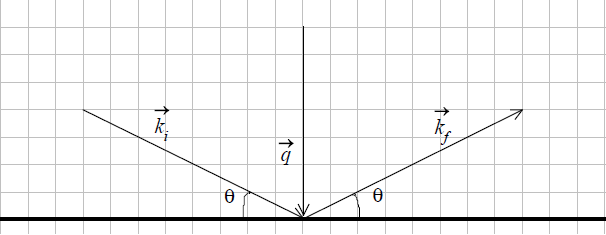
\includegraphics[width=0.7\textwidth]{billede3.png}
\caption{En neutron der laver totalrefleksion på et neutronspejl}
\end{figure}

Når vi arbejder med guides, er vi ofte interesseret i den kritiske vinkel, hvilket er den størst mulige vinkel, hvorved vi kan få totalrefleksion mellem guide og neutron. Når vi har totalrefleksion, gælder det at længden af $\vec{k_i}$ er lig længden af $\vec{k_f}$, hvilket vi blot vil kalde for k:
\begin{align}
k_i=k_f=k
\end{align}
(Noter, at vi blot skriver længden af $\vec{k_i}$ og $\vec{k_f}$ som $k_i$ og $k_f$) \\
Når vi ved dette, kan vi ved hjælp af simpel trigonometri skrive længden af $\vec{q}$ som:
\begin{align} \label{eq:q1}
q=2k \cdot sin(\theta)
\end{align}
Hvor $\theta$ er vinklen som neutronen bliver reflekteret med. Hvis vi gør brug af vores definition af $k$, får vi at ligning (\ref{eq:q1}) kan skrives som:
\begin{align} \label{eq:q2}
q=4\pi \cdot \frac{sin(\theta)}{\lambda}
\end{align}
Hvor $\lambda$ altså er bølgelængden for neutronen. Da vi har ved små vinkler at gøre, kan vi approksimere ligning (\ref{eq:q2})  ved $sin(\theta)≈\theta$. Vi får at:

\begin{align}
q≈4\pi \cdot \frac{\theta}{\lambda}
\end{align}

Som sagt er det ofte relevant, at kigge på den kritiske vinkel, hvilket altså er den størst mulige vinkel, hvorved totalrelfleksion er mulig. Denne vinkel betegner vi som $\theta_c$. Når vi har totalrefleksion ved den kritiske vinkel, har vi en kritisk spredningsvektor, hvis længde vi betegner med $q_c$. For et givent materiale er $q_c$ konstant, og vi ser derfor, at den kritiske vinkel er en funktion af bølgelængden. Vi får at:

\begin{align}
q_c≈4\pi \cdot \frac{\theta_c(\lambda)}{\lambda}
\end{align}

Vi har, at værdien for den kritiske spredningsvektor for nikkel er $q_{c, Ni}=0.0217\text{Å} ^{-1}$ \cite{lefmann_arleth_kirkensgaard_lebech_thomsen}. Dette er en fast værdi for nikkel, og vi kan dermed let udregne den kritiske vinkel som funktion af neutronens bølgelængde som: 

\begin{align}
\frac{q_{c,Ni} \cdot \lambda}{4\pi}=\theta_c(\lambda)
\end{align}

Vi får hermed ved simpel indsætning, at neutroner med en bølgelængde på 1Å har en kritisk vinkel på omtrent $0.1^∘$, mens neutroner med bølgelængde på 10Å har en kritisk vinkel på omtrent $1^∘$, på et neutronspejl lavet af nikkel.
Man kan dog opnå en højere værdi af $q_c$ ved at lægge lag af andre materialer, mellem lagene af nikkel. Denne værdi af $q_c$ udregnes som:

\begin{align}
q_c=m \cdot q_{c,Ni}
\end{align}

Hvor m er den såkaldte m-værdi. Denne er altså en indikation på, hvor stor en kvalitet spejlet har, i forhold til et rent Ni-spejl. m-værdien for et spejl er ofte på et par stykker, men kan komme helt op på 7. \cite{lefmann_arleth_kirkensgaard_lebech_thomsen}

Neutronspejle består af et nedre lag af såkaldt $substrate$. Dette er basis for spejlet, og kan laves af flere forskellige materialer, alt afhængigt af, hvor stor kvalitet spejlet ønskes i, og hvordan spejlet skal interergere med neutronerne. Derudover består neutronspejle af nogle lag $coating$ ovenpå. Det er netop denne coating der dikterer m-værdien for spejlet, dvs. mange lag coating giver en høj m-værdi. Senere vil vi komme ind på priserne for henholdsvis substrate og coating, da det er en vigtig begrænsing for vores simuleringer.

\subsubsection{Elliptiske guides}
Når man samler en række neutronspejle i forlængelse af hinanden, kalder man det for en neutronguide. De simpleste guides er selvsagt fuldstændig lige. Dette er dog ikke altid det mest hensigtsmæssige. Der kan være flere forskellige grunde til, at man vil have en enten kurvet eller eliptisk guide. 
Hvis neutronerne skal transportereres store afstande, kan det være en fordel, at gøre guiden breddere, ved at gøre den enten eliptisk, eller delvis eliptisk i starten. Derved kommer der længere flyvetid mellem hvert sammenstød mellem neutronen og guiden, og færre neutroner går dermed tabt. 
Derudover kan en eliptisk guide opnå en større brilliance transfer, end en almindelig lige guide. Dette skyldes at færre neutroner går tabt lige  i starten, men at nogle af neutronerne tilgengæld har en større divergens når de kommer hen til prøven. Dette ses tydeligt i vores resultat afsnit.

Det kan også være en idé i, at få den prøve man skyder på, uden for synslinje af neutronkilden, således at man ikke får baggrundsstråling fra kilden. Dette kan gøres ved enten at lave en kurvet guide, eller eventuelt lave et såkaldt 'kink'. Et kink består af et neutronspejl, der reflekterer neutronerne fra en guide til en anden, så man kan få en vinkel mellem sine to neutronguides. 
Det kan også være nødvendigt at samle guiden på visse steder. Dette kan eksempelvis være nødvendigt, hvis man vil indsætte en såkaldt chopper.

\subsubsection{Chopper}
En chopper er en roterende komponent, der kun lader neutroner passere i visse tidsintervaller. Den simpleste chopper er en 'disk chopper', som basalt set er en roterende disk, med et antal 'revner' eller huller nær kanten. Chopperen bliver sat til at rotere foran neutronstrålen, og neutronerne kan dermed kun passere chopperen, når chopperen er åben, dvs. når neutronen kan passere gennem hullet i chopperen. I det chopperen roterer, vil det kun til nogle tidspunkter være muligt for neutronerne at passere. Med en chopper kan man altså opdele neutronstrålen i mindre bider. Dette kan give en bedre kontrol over neutronerne, og dermed bedre resultater. \cite{ess_folder}

\subsubsection{Neutronkilder, moderator og neutrondetektionr}
Neutroner kan genereres på flere forskellige måder. Ved ESS i Lund bliver neutronerne frembragt ved protonbombardament af en wolframkilde. Alle neutronerne skal helst have samme hastighed, og for at give dem dette gør man brug af en såkaldt moderator. En moderator er et ofte hydrogenholdigt materiale, som omkrænser neutronkilden. Neutronernes energi bliver derved normaliseret ved, at de langsomt vil opnå termisk ligevægt med moderatoren gennem sammenstød med moderatorens hydrogenatomer (eksempler på moderatorer kunne være $H_2O$, $H_2$ eller $CH_4$). Man kan hermed ændre på neutronernes energi ved at ændre på moderatorens temperatur. 
Efter neutronerne har interergeret med prøven, skal de selvsagt detekteres, således at man kan få forsøgsresultater. Neutronerne 
bliver ofte detekteret gennem en kerneprocess med helium, hvorefter der bliver frigjort noget energi, $Q$. \cite{lefmann_arleth_kirkensgaard_lebech_thomsen}

\begin{align}
^3He + n \to  ^3H + ^1H + Q
\end{align}

Den frigivne energi, $Q$, giver anledning til et elektrisk signal, og neutronen er dermed blevet detekteret.


\subsection{Krav til guidesystemerne}
De forskellige guides der bliver bygget, skal bruges til forskellige eksperimenter, hvorfor deres specifikationer er forskellige. BIFROST som bearbejdes i dette projekt må koste op til 2.10 M€, hvilket selvfølgelig har betydning for vores optimeringsmuligheder. Prøven skal befinde sig 165m fra kilden, og derfor skal selve guiden være 162,4m lang, da de første 2m og de sidste 0.6m skal være fri for guides, så det er plads til diverse instrumenter. Endvidere må guiden højst have en tykkelse på $10cm \cdot 10cm$ på sit breddeste, for at mindske prisen.
\\
Derudover er der krav til det substrate, som neutronspejlene blandt andet er lavet af. De første 23.5m guide skal have substrate bestående af aluminium, hvilket koster (omtrent) $25.000 \text{€}/m^2$. Det er nødvendigt med aluminium substrate det første stykke, da strålingen er meget høj og denne ikke ioniserer aluminium på samme måde som f.eks. kobber. Hvis noget går i stykker kan man derfor stadig komme ind og lave det igen. Efter de første 23.5m guide, kan man skifte til en billigere substrate, bestående af borcron, hvilket koster (omtrent) $14.000 \text{€}/m^2$.
\\
Man skal også gøre sig overvejelser mht. de tidligere nævnte m-værdier. Selve materialet til coating af spejlene er ikke videre dyrt, men coatingsprocessen får prisen til at stige. Basisprisen for coating er (omtrent) $L\cdot8(K\text{€}/m)$, hvor L er længden du vil dække med coating. Ekstra lag koster endda (omtrent) $(L\cdot(m^{2,6})/4)\cdot2(K\text{€}/m)$, , hvor L er længen du vil dække, og m er m-værdien for spejlet. Derfor bruger man kun høje m-værdier i begrænset omfang. De steder man bruger høje m-værdier er hvor flere neutroner rammer i en større vinkel, da en høj m-værdi øger muligheden for at reflektere ved højere indgangsvinkler. Derfor bruges de ved starten og slutningen af hver del. Selv hvis man havde råd til en høj m-værdi i hele stykket, ville man ikke gøre det,da en høj m-værdi udelukker nogle neutroner, der ellers ville nå frem til prøven.
\\
Udover prisen som en begrænsende faktor, skal der indsættes choppers 0.5m og 23.5m inde i vores guide. Det resulterer i, at guidens tværsnitsareal skal sænkes på disse steder, så den stemmer overens med chopperne. Dimensionerne af guiden omkring en chopper skal være på $3cm\cdot5cm$. 
\\
Divergensen i vores guide må højst fluktuere med $\pm0.75^\circ$. Derudover er det vigtigt for eksperimentet, at neutronerne har den rette energi, hvilket er en af grundene til, at prøven skal være uden for synslinje af kilden. Hvis prøven ikke er dette, kan enkelte hurtige neutroner blot  bevæge sig direkte hen til prøven, uden at blive reflekteret. Dermed ville vi ikke have nogen kontrol over disse neutroner.
\\
Målet er derefter at nå så høj brilliance transfer som muligt i et bølgelængdeinterval indenfor 0.5Å til 8Å.

\subsection{Bedømmelse af guidesystemer}

Når man har lavet sin simulering i MCstas, er det klart at man skal bedømme hvorvidt ens guide er god eller ej. I MCstas kan man let indsætte forskellige monitors foran sin prøve, så man kan se, hvordan neutronerne rammer prøven. Blandt monitors vi har brugt er blandt andet monitors der er følsomme overfor positionen hvormed neutronerne rammer prøven, bølgelængderne af neutronerne, divergensen for neutronerne (altså indfaldsvinklen hvormed neutronerne rammer prøven), og brilliance sensitive monitors. Specielt bedømmer vi vores guides på baggrund af hvor meget af brilliancen de bevarer, dvs. hvor høj en brilliance transfer de har. Vi er dog også kritiske overfor den brilliance transfer vi får. Det er vigtigt, at vores brilliance transfer er høj, for de rigtige bølgelængder. Derudover bedømmer vi også vores guides på baggrund af deres pris. Prisen er den eneste variabel der begrænser brugen af vores m-værdier, så for at få en realistisk guide, er det vigtigt at have prisen med som variabel.


\subsection{Optimering}
Vi har arbejdet med flere forskellige guides, som vi har forsøgt at optimere mest muligt. Vi har gjort dette ved at parametrisere vores instrumenter, således at vi let kunne ændre på geometrier og m-værdier. På baggrund af vores simuleringer, har vi skabt et optimeringsprogram, som kunne benytte parametriseringen af instrumentet, til automatisk at finde værdien af de parametre, der gav bedst muligt resultat.
Senere forsøgte vi også at tage højde for m-værdiernes pris, så vi kunne få en god mellemvej mellem pris og kvalitet af m-værdier. Vi har altså basalt set optimeret på geometri, m-værdi og pris. 

Alt dette er i første omgang bedømt på baggrund af arealet under vores brilliance transfer kurve, ved bølgelængder mellem 0.5Å og 8Å. Derefter har vi også kigget på, om vores optimeringer overholder eksempelvis pris-og divergenskrav. I vores script har vi eksempelvis taget højde for, at det ikke er godt, at få en høj brilliance transfer, hvis mange af neutronerne kommer med en divergens større end $\pm0.75^\circ$. Derfor kan vores optimering give os et godt bud på, hvordan en god og realistisk neutronguide kunne se ud. 


\section{Resultater}

\subsection{Vores guide(s)}
Vi har i løbet af dette projekt lavet en del virtuelle eksperimenter vha. MCStas. Vi vil dog begrænse os til nogle enkelte guides, for at begrænse omfanget af rapporten.

Specifikt vil vi fokusere på disse simuleringer:
\begin{enumerate}
    \item Simpel simulering af lige versus elliptisk guide \cite{github:st_vs_el}
    \item Simpel simulering af elliptisk guide der minder om ESS forholdende. \cite{github:ess_sim_simple}
    \item En mere realistisk simulering af potentiel ESS guide geometri. \cite{github:ess_brill_optimized}
\end{enumerate}

\subsubsection{Sammenligning af lige og elliptisk guide}
Denne simulering blev fremstillet for at fremhæve forskellen mellem en lige guide, og en elliptisk guide. En skitse af deres geometri ses herunder:

\begin{figure}[H]
\centering
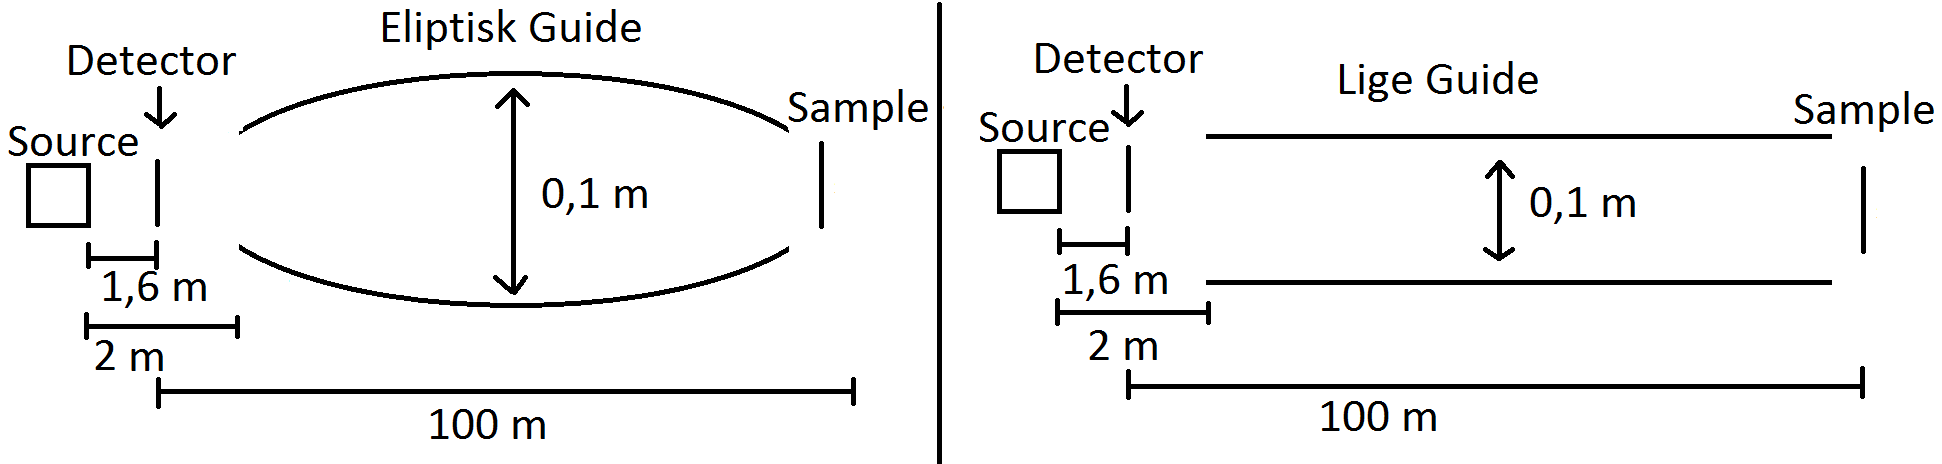
\includegraphics[width=1\textwidth]{Straight_VS_Elipse.png}
\caption{Eksempel på guidegeometrien, den lige guide består kun af de lige streger, mens den eliptiske kun består af de eliptiske streger}
\end{figure}

Hvis du plotter resultaterne, er der en tydelig forskel mellem den eliptiske og lige guide. Resultatet ses herunder:

\begin{figure}[H]
\centering
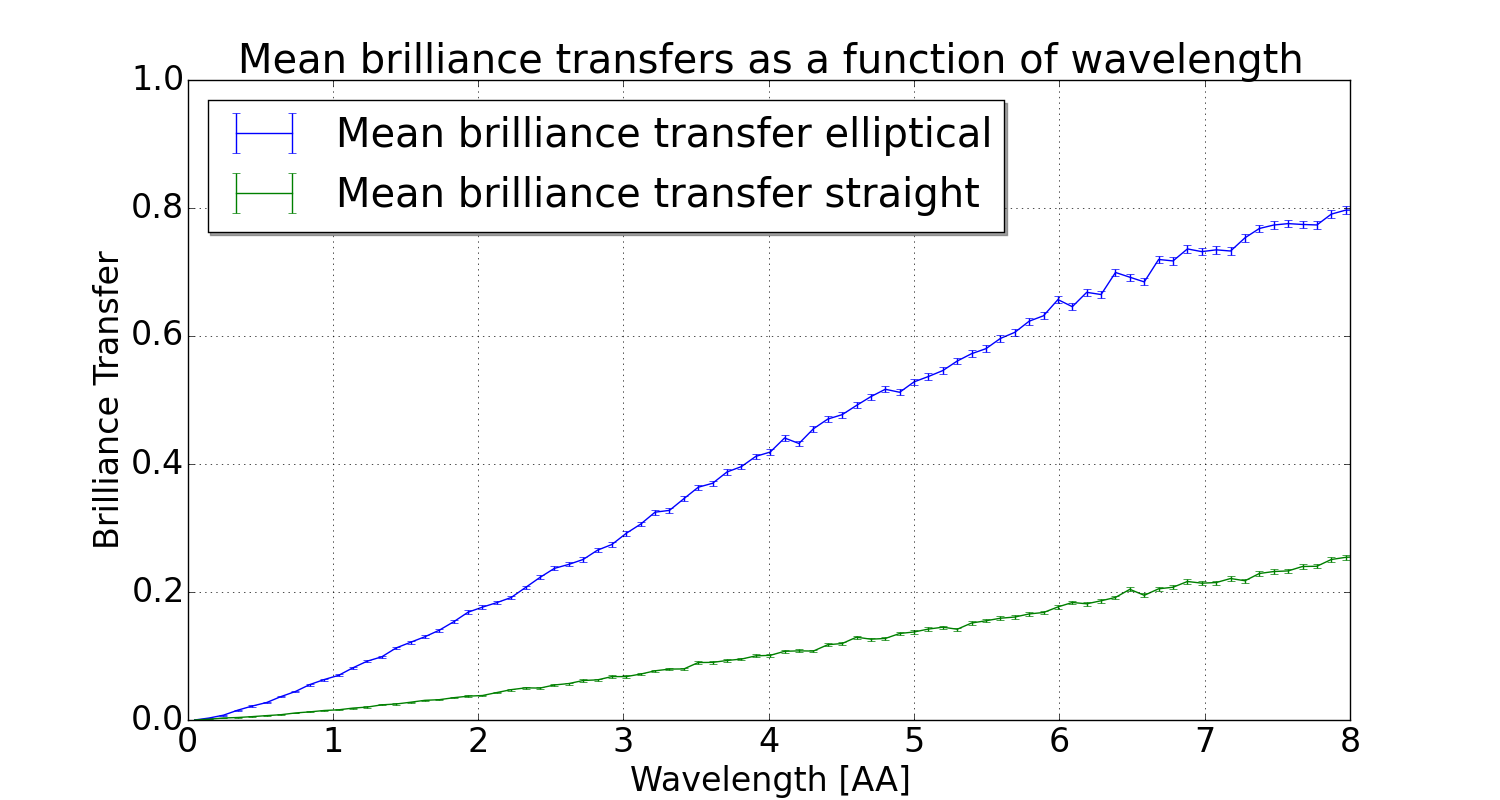
\includegraphics[width=1\textwidth]{st_vs_elip_148950055477097.png}
\caption{Brilliance transfer som funktion af bølgelængden for lige og eliptisk guide}
\end{figure}


\subsubsection{Det simpleste ESS tilfælde}
Denne guide blev fremstillet for at simulere det simpleste tilfælde man kan forestille sig ved ESS. Vi har kun her optimeret efter de simpleste omstændigheder. Dvs. vi har sat en høj fast m-værdi, og derefter optimeret guidens geometri, hvor den skulle overholde nogle af de simpleste geometriske krav.
En skitse af guidens geometri ses herunder:

\begin{figure}[H]
\centering
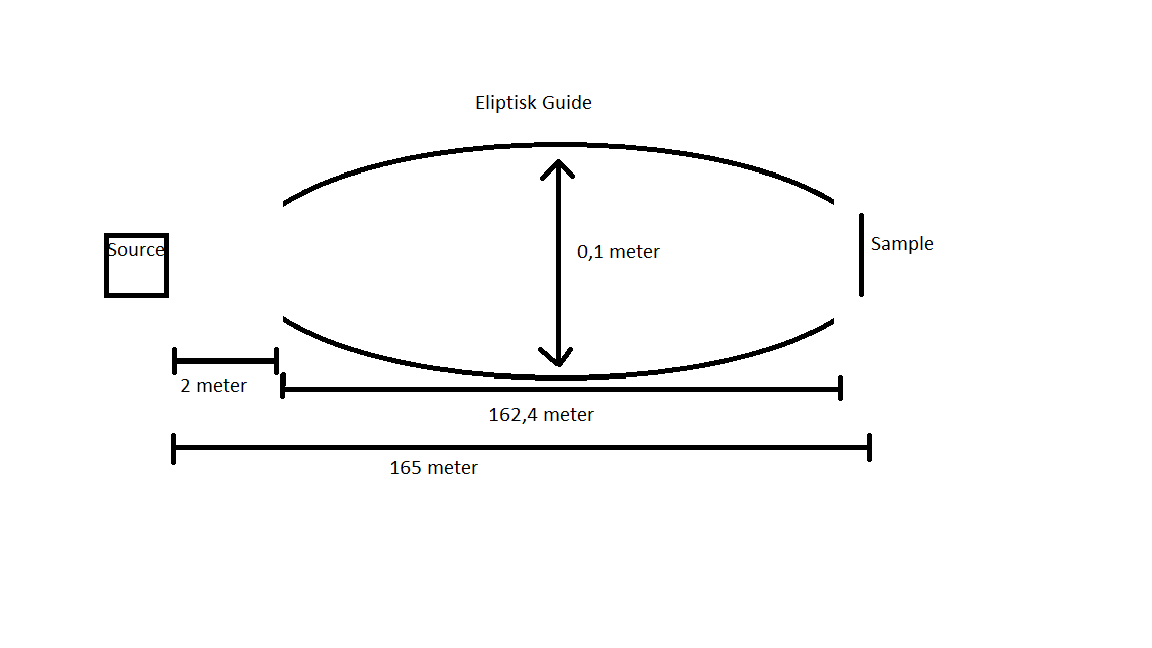
\includegraphics[width=1\textwidth]{Elipse.png}
\caption{Skitse af simpel eliptisk guidegeometri}
\end{figure}

Når vi plotter vores optimerede guide, får vi følgende brilliance transfer som funktion af bølgelængden:

\begin{figure}[H]
\centering
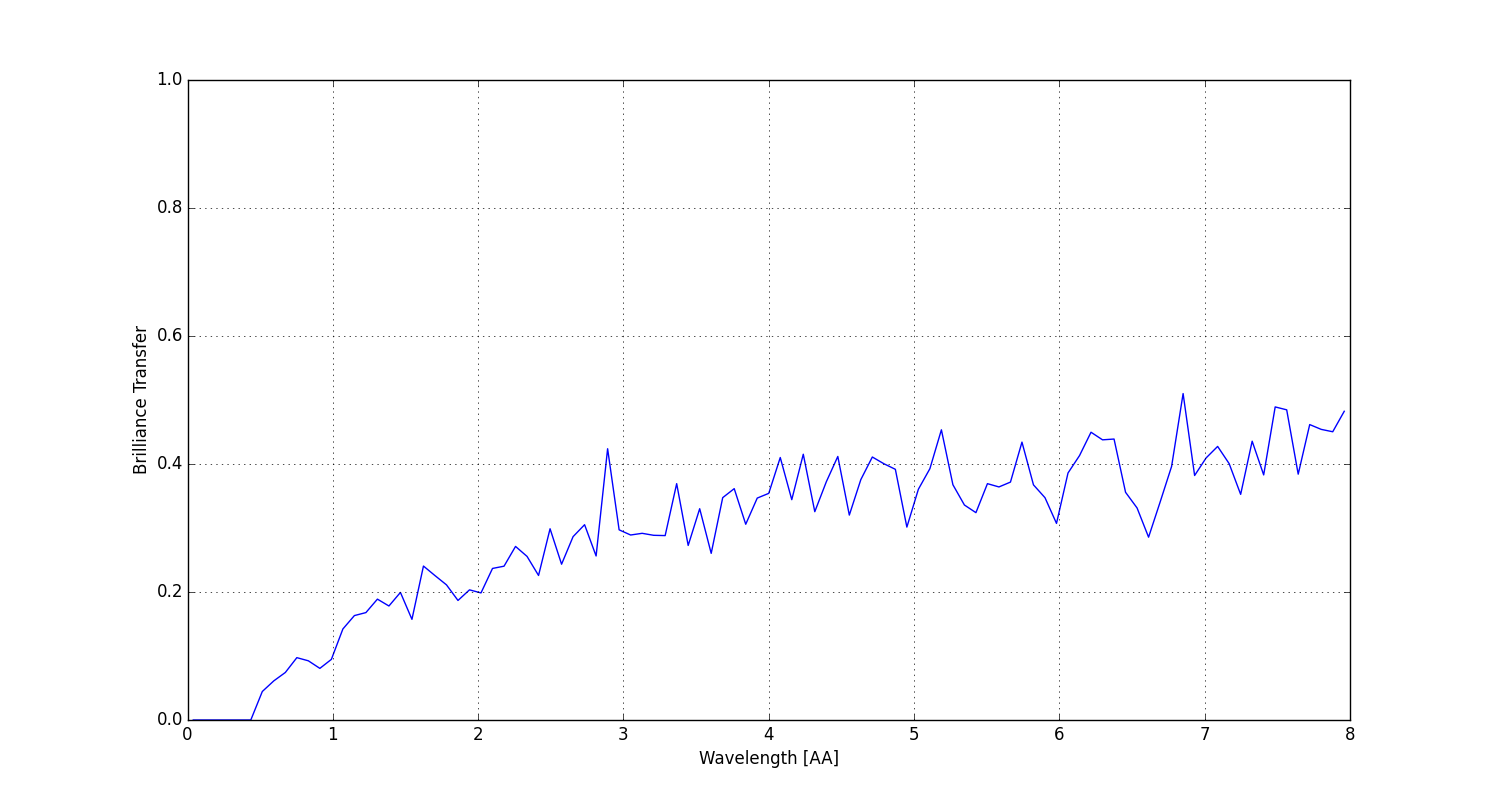
\includegraphics[width=1\textwidth]{optimized_mean_4.png}
\caption{Brilliance transfer som funktion af bølgelængden for simpel eliptisk guide.}
\end{figure}




\subsubsection{Realistisk ESS geometri}
Denne guide tager udgangspunkt en guidegeometri som har været under overvejelse til forsøget på ESS. Guidens geometri bliver populært kaldt 'EGCGE', dvs. den består af en eliptisk guide (E), et gab (G), en kurvet guide (C), endnu et gab (G), og til sidst en eliptisk guide igen (E). En skitse af guiden er tegnet herunder:

\begin{figure}[H]
\centering
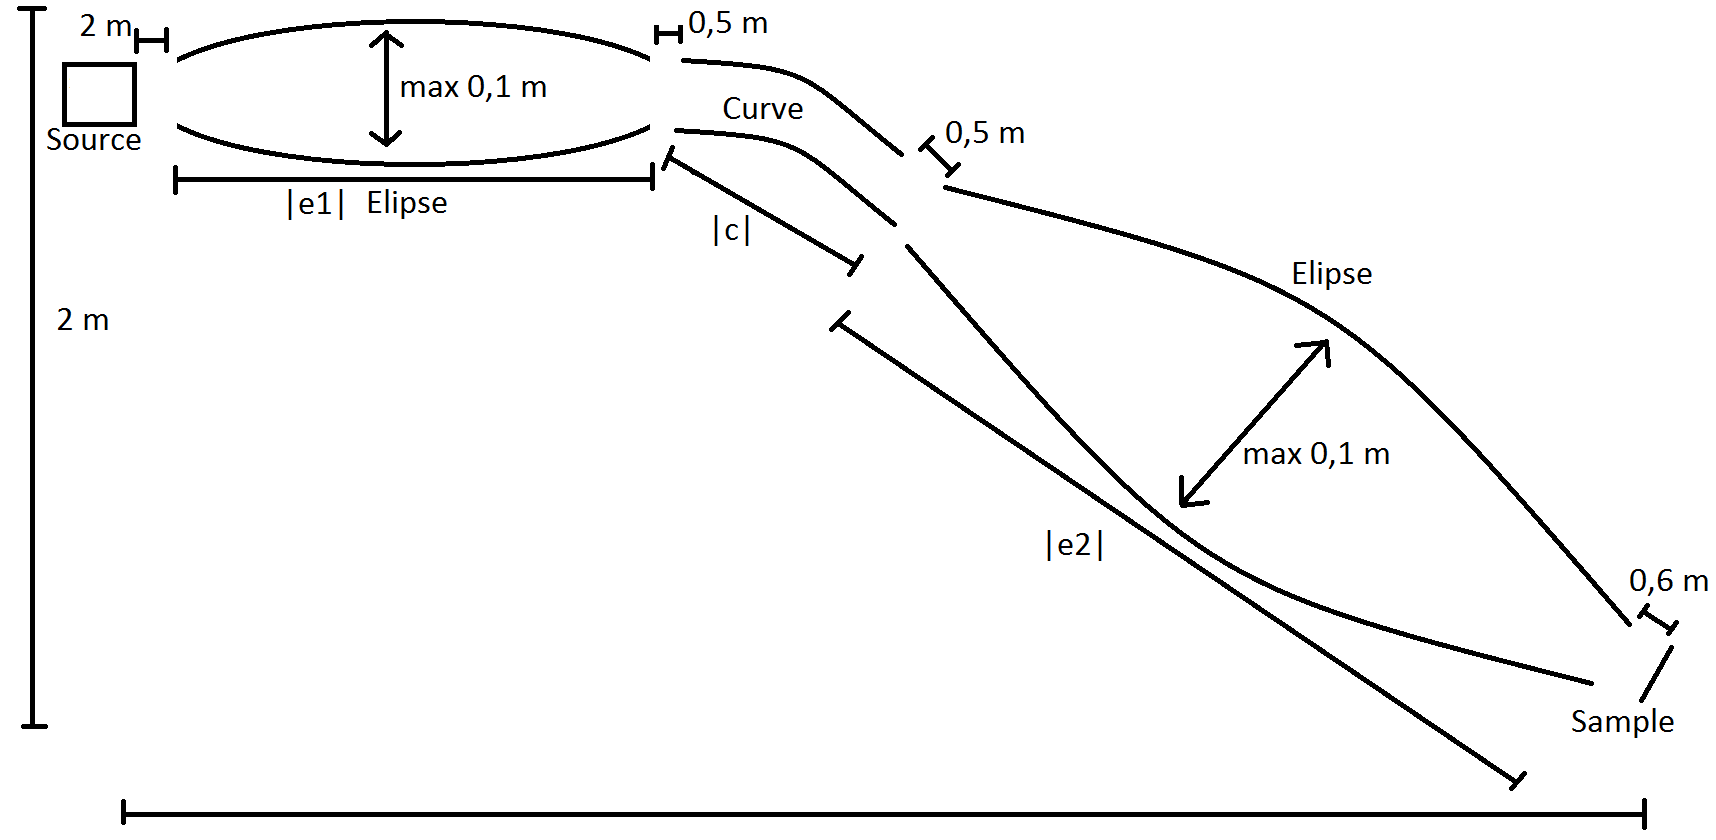
\includegraphics[width=0.5\textwidth, angle=90]{EGCGE.png}
\caption{Skitse af realistisk ESS geometri}
\end{figure}

Dette er en guidestruktur som potentielt godt kunne blive brugt ved ESS. Vi har optimeret med hensyn til geometrien. Vores resultat ses herunder

\begin{figure}[H]
\centering
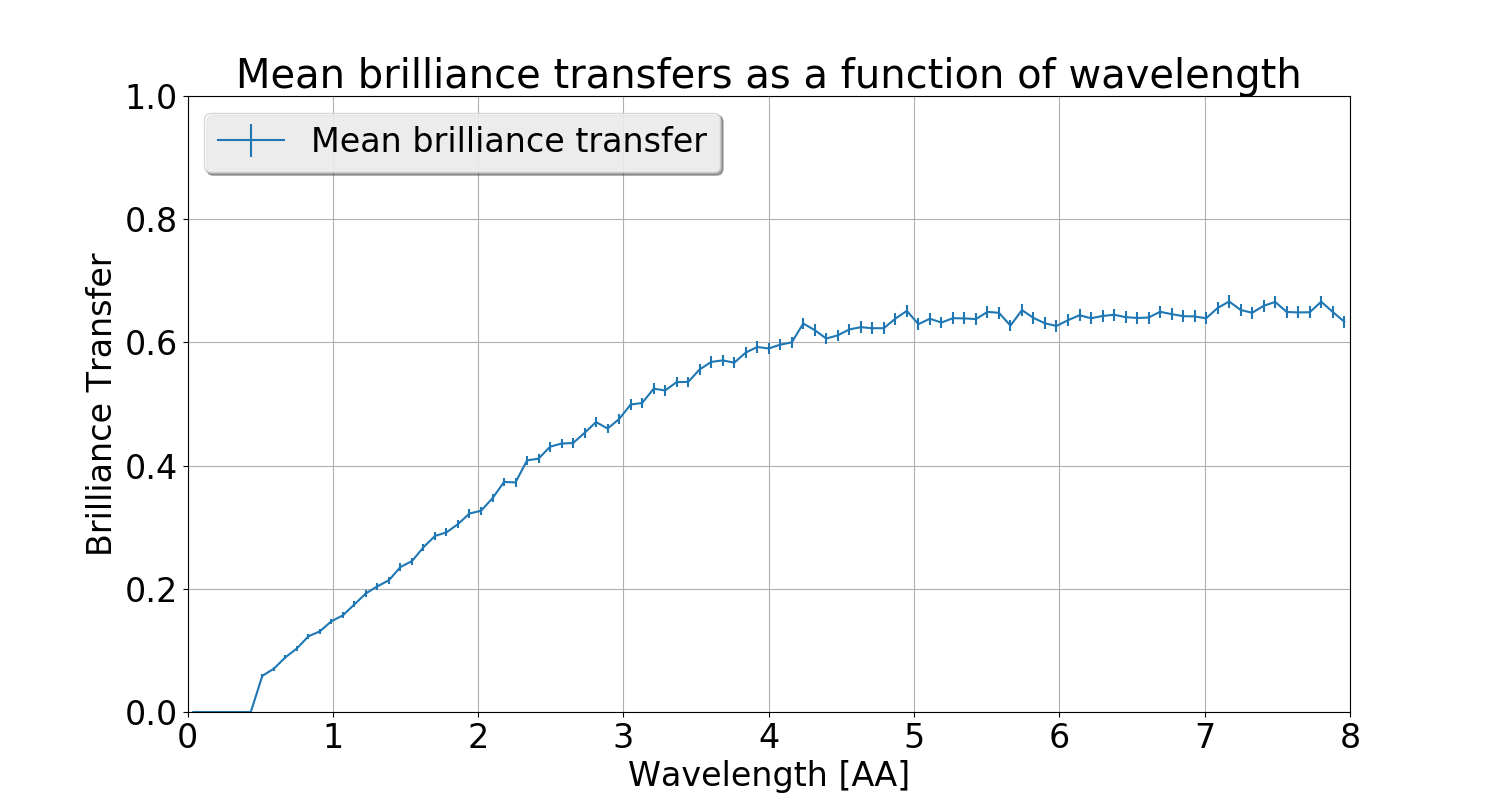
\includegraphics[width=1\textwidth]{brill_optimized_mean_148952691102106.png}
\caption{Brilliance transfer som funktion af bølgelængde af optimeret EGCGE}
\end{figure}


\section{Diskussion}

\subsection{Bedømmelse af vores guides}
I vores første simulering hvor den lige guide blevet plottet mod den eliptiske guide, var det meget tydeligt, at den eliptiske gav en klart større brilliance transfer. Dette er første tegn på, at guidegeometrien kan optimeres. Dog må vi huske, at det ikke kun er brilliance transfer, der tæller. Divergensen betyder eksempelvis også meget. Vi kan se på figur \ref{ap:div_straight_after} og \ref{ap:div_ellipse_after} at den elliptiske guide har betydeligt større divergens, end den lige guide. Hvis du optimere din guide kun efter brilliance transfer, kan det altså komme til at koste i divergens. Vi kan se, at hvis vi har et krav på $\pm 0.75^\circ$, er dette kun opfyldt til fulde ved den lige guide. Der er flere måder at komme uden om dette problem på. Eksempelvis kunne man fra start optimere sin guide med et krav om en divergens på maks  $\pm 0.75^\circ$, eller man kunne gøre brug af choppers eller pinholes. Derudover får vi i både vores lige og eliptiske guides, meget støj, fordi prøven ligger i direkte synslinje til kilden. Dermed kommer der nogle hurtige neutroner direkte fra kilden til prøven. Dette viser også tegn på, at simple geometrier, som eksempelvis en enkelt ellipse, ikke altid er den bedste mulighed.
\\
\\
For at opfylde divergenskrav samt at få prøven ud af direkte synslinje af for at reducere støj introducerer vi en ny, mere kompleks, geometri. Den mere komplekse geometri (EGCGE) sikrer at vi vha. choppers og pinholes kan reducere divergensens for at opfylde divergenskravet samt at fjerne neutroner med for høj energi. Vi har derfor optimeret på den mere komplekse geometri som under de optimale forhold har meget lille tab af brilliance transfer.
\\
\\
Den første fejlkilde i vores vurdering af systemet er udefrakommende neutroner, disse er meget svære at simulere da de både kan komme fra andre eksperimenter, men og fra passiv støj. En anden almindelig fejlkilde er fabrikations fejl i spejlene, dette kan være ujævnheder på overfladen eller fejl i placering af spejlene. Over tid øges fejlen også da neutronerne bliver absoberet af substratet som leder til ionisering af substratet hvilket både kan give ekstra baggrundstråling og lede til opbygning af gas i substratet som giver ujævnheder i overfladen. Til sidst er der naturligvis fejl i vores detektorer, som ikke kan opfange alle neutroner.
\\
\\
Eksperimentet kan naturligvis også forbedres, dette kunne f.eks. være ved at afprøve nye, bedre, geometrier. Herudover har vi haft en begrænset mængde tid til optimeringerne, derfor er det muligt at vi kun har fundet et lokalt maksimum for brilliance transfer frem for det globale. Derudover har vi arbejdet med optimeringen i faser. Først har vi optimeret på geometrien af opsætningen hvorefter, vi har haft fokus på m-værdier og pris af opstillingen. Det er derfor muligt, at vi ikke har fundet det optimum som både tager højde for pris og geometri, men derimod et lokalt maksimum for kombinationen af disse paramtre.

\section{Konklusion}
Vi har gennem dette projekt fundet en geometri, samt parametrene til denne geometri, der opfylder alle krav til neutronguiden, med undtagelse af pris, der har en meget pæn overførsel af neutronerne. Vi har også defineret begreber og målstørrelser til vurdering af disse geometrier. Herudover har vi diskuteret relevante problemstillinger med både Monte Carlo simuleringer generelt, men også problemer i vores specifikke simulering. Vi har også fremstillet et computerprogram til automatisk at optimere på parameteriserede simuleringer for at lette arbejdsbyrden i designet af instrumenterne.


%% Rapporten er slut! %% 
\newpage
%% Kilder %%
\addcontentsline{toc}{section}{Litteratur}
\bibliographystyle{ieeetr}
\bibliography{sources} 

%% Kilder er slut! %% 
\newpage
%% Appendix %%

\appendix
\section{Appendix}

\subsection{Sammenligning af lige og elliptisk guide}

\begin{figure}[H]
\centering
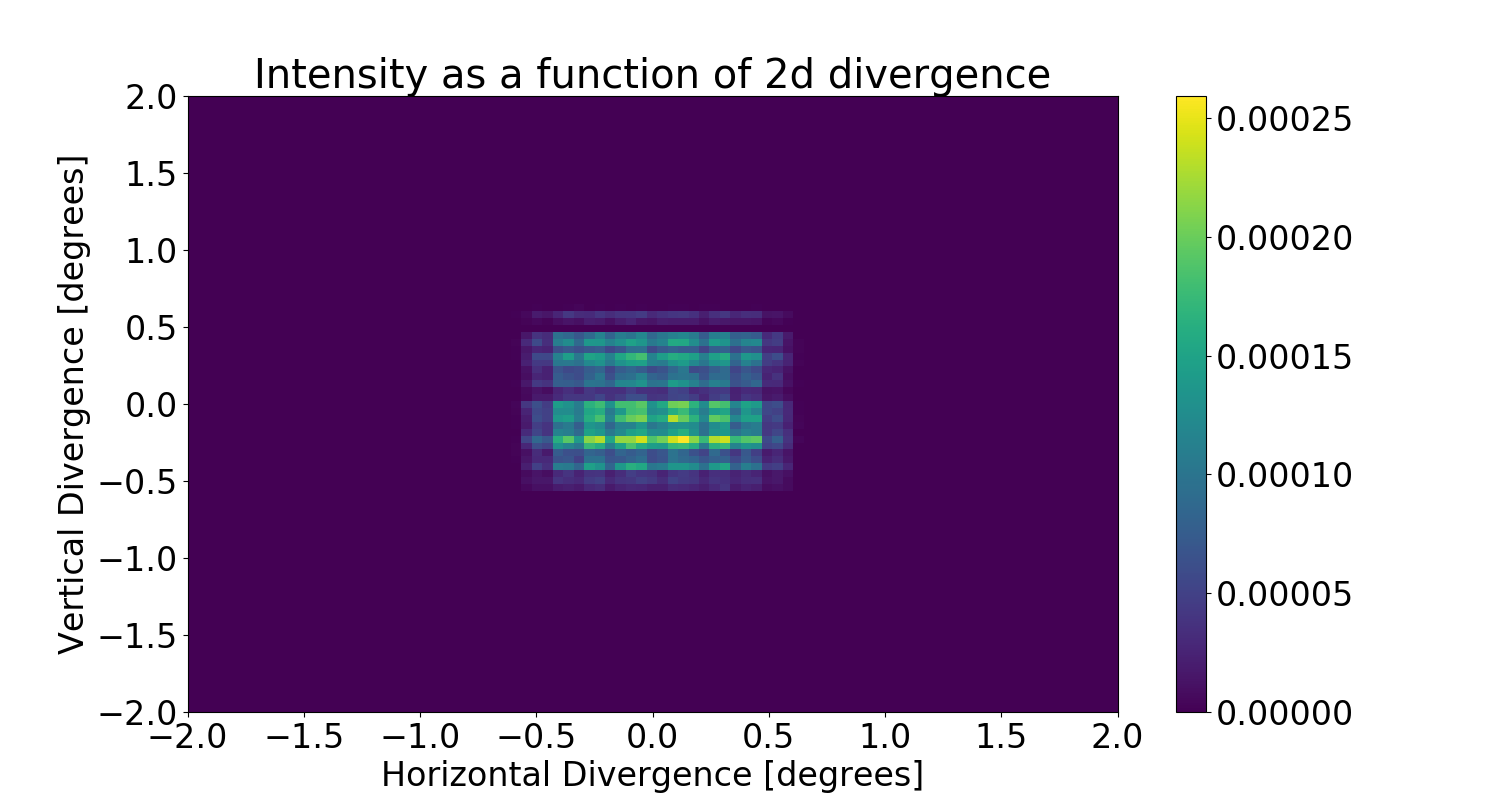
\includegraphics[width=1\textwidth]{div_straight_after.png}
\caption{Divergensen efter den lige guide}  \label{ap:div_straight_after}
\end{figure}


\begin{figure}[H]
\centering
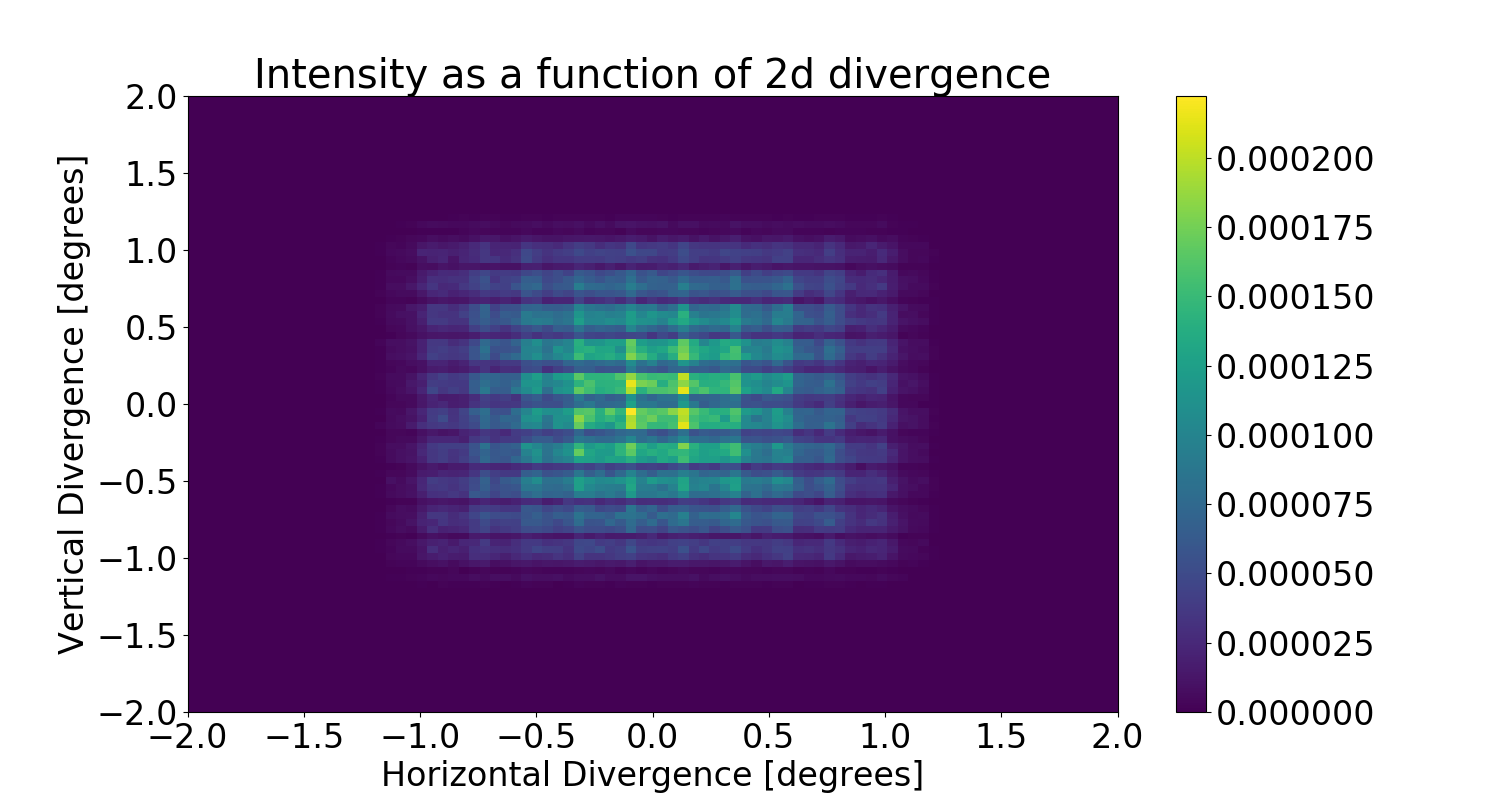
\includegraphics[width=1\textwidth]{div_ellipse_after.png}
\caption{Divergensen efter den eliptiske guide} \label{ap:div_ellipse_after}
\end{figure}


\begin{figure}[H]
\centering
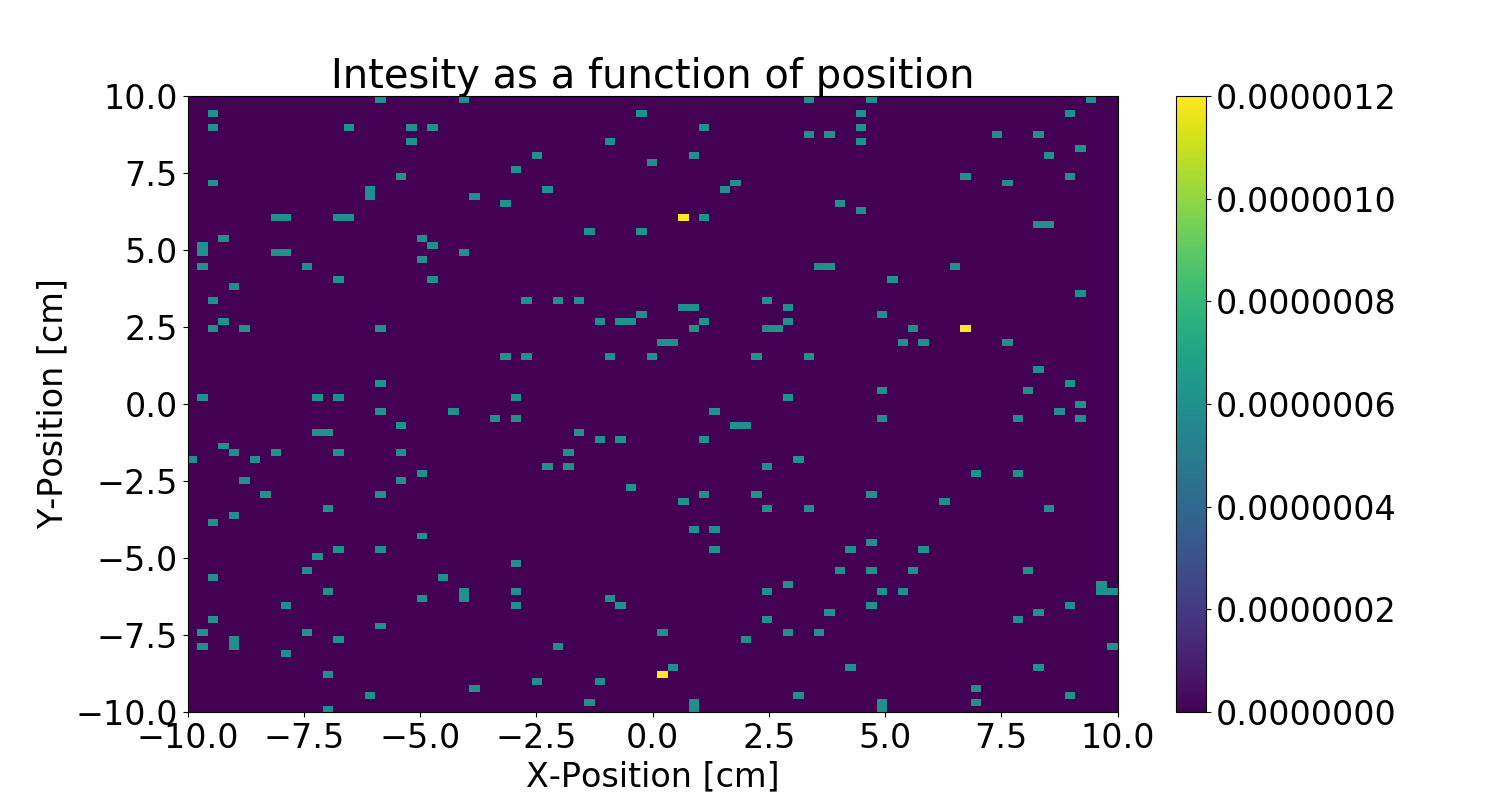
\includegraphics[width=1\textwidth]{psd_straight_after.png}
\caption{Positionen af neutronerne efter den lige guide}
\end{figure}

\begin{figure}[H]
\centering
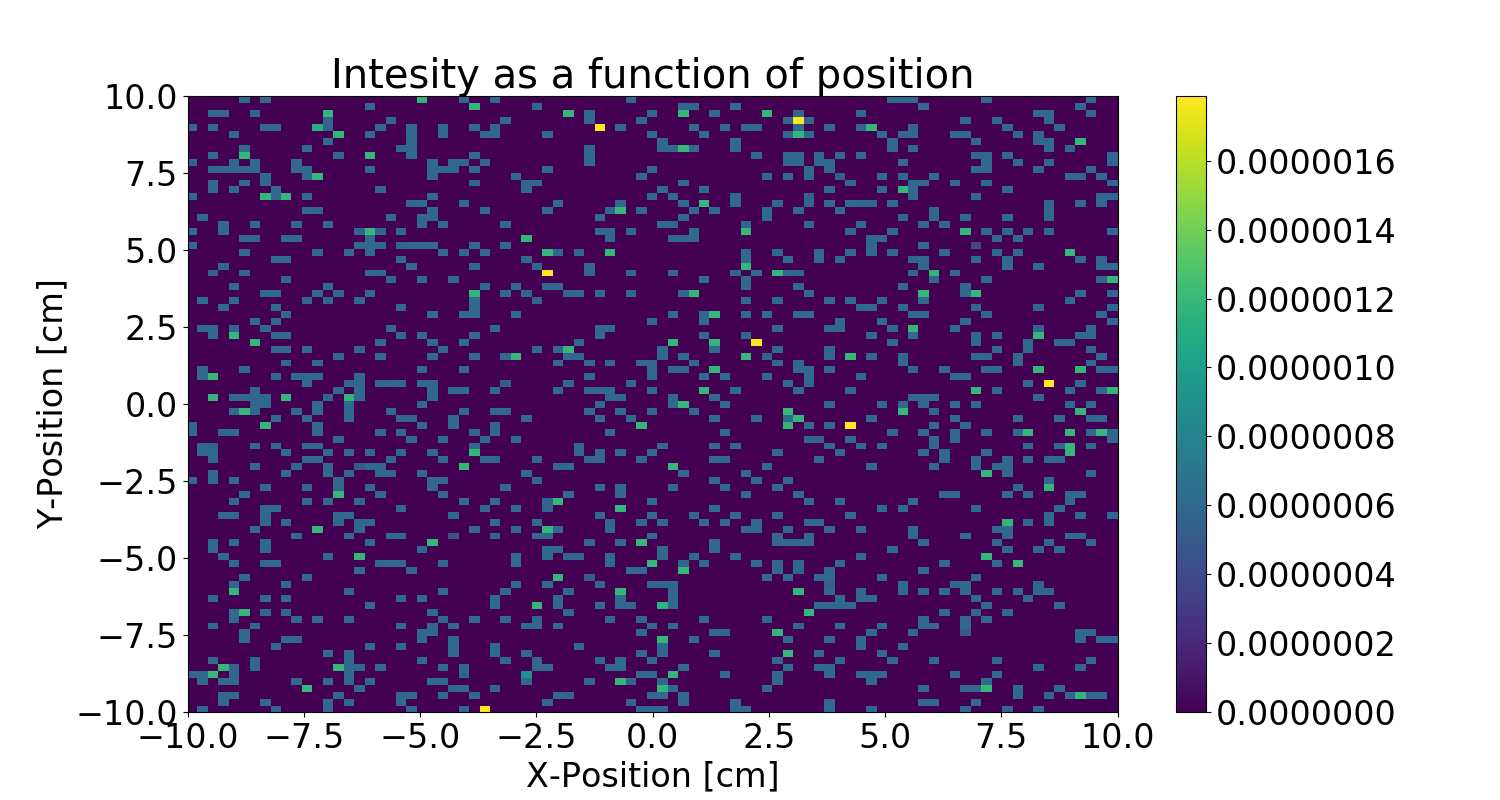
\includegraphics[width=1\textwidth]{psd_ellipse_after.png}
\caption{Positionen af neutronerne efter den eliptiske guide}
\end{figure}



\begin{figure}[H]
\centering
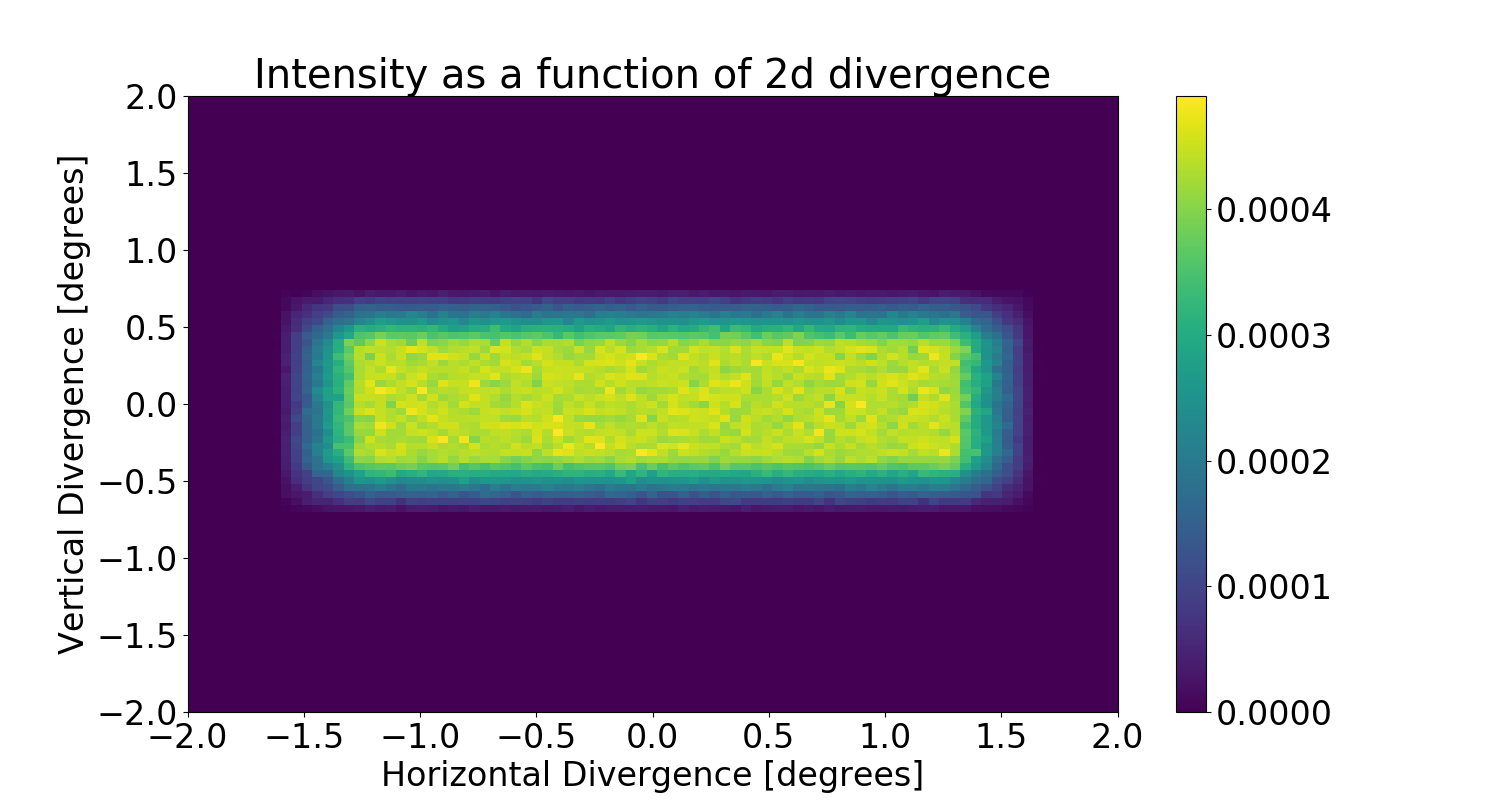
\includegraphics[width=1\textwidth]{div_straight_before.png}
\caption{Divergensen inden guiden}
\end{figure}

\begin{figure}[H]
\centering
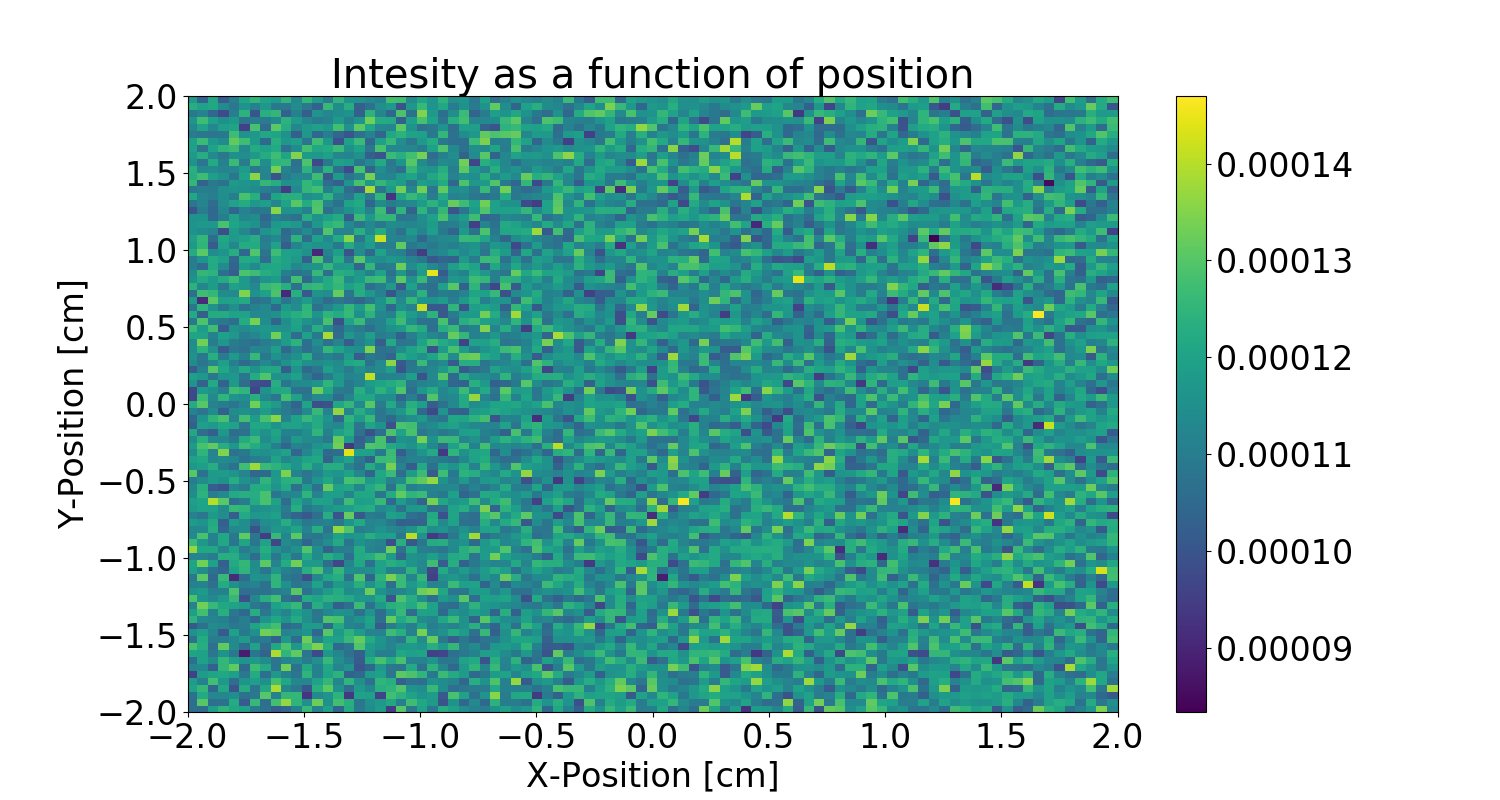
\includegraphics[width=1\textwidth]{psd_straight_before.png}
\caption{Positionen af neutronerne inden guiden}
\end{figure}



\subsection{Det simpleste ESS tilfælde}

\begin{figure}[H]
\centering
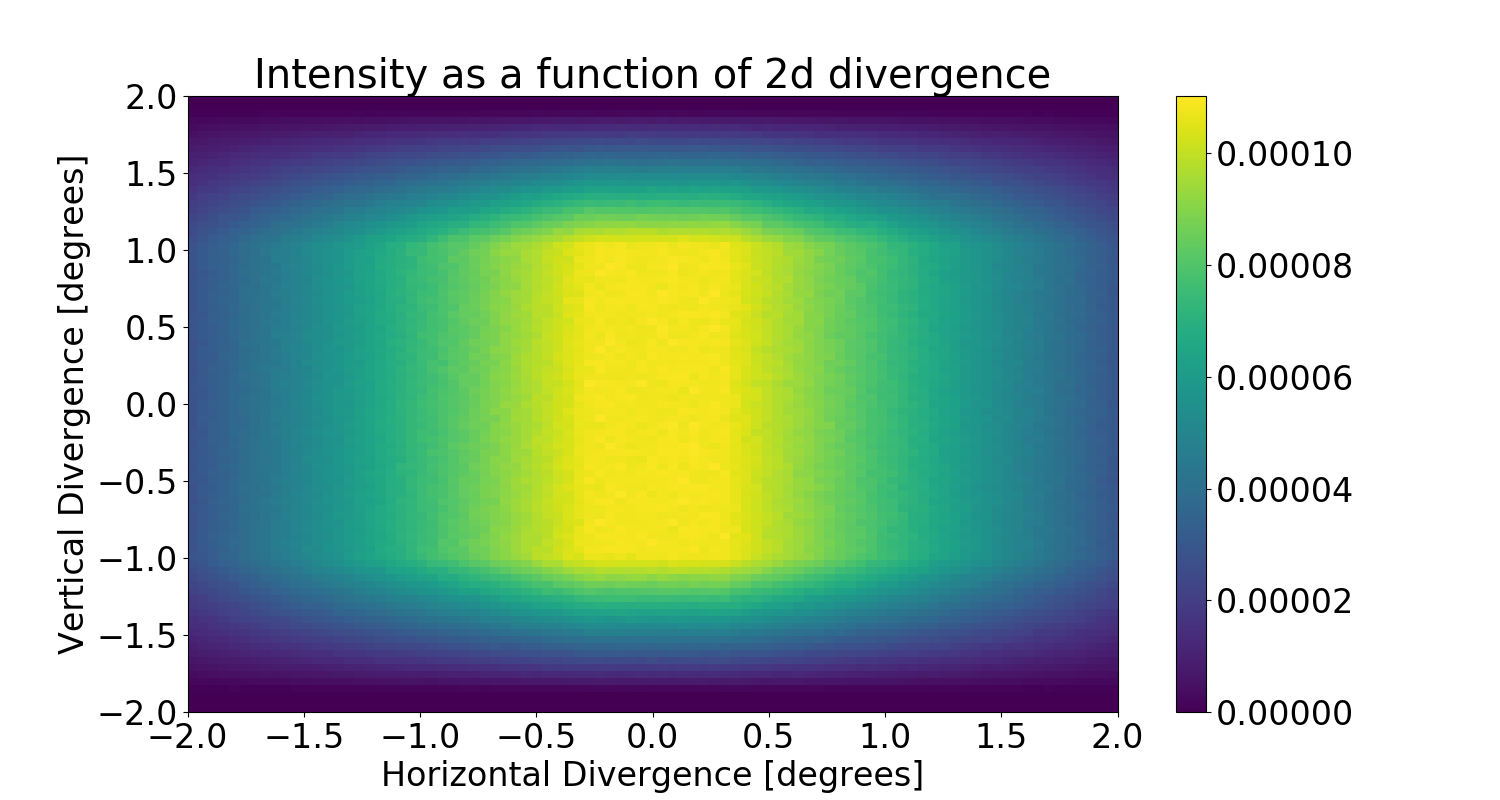
\includegraphics[width=1\textwidth]{div_ess_simple_after.png}
\caption{Divergens efter den simple ESS guide}
\end{figure}


\begin{figure}[H]
\centering
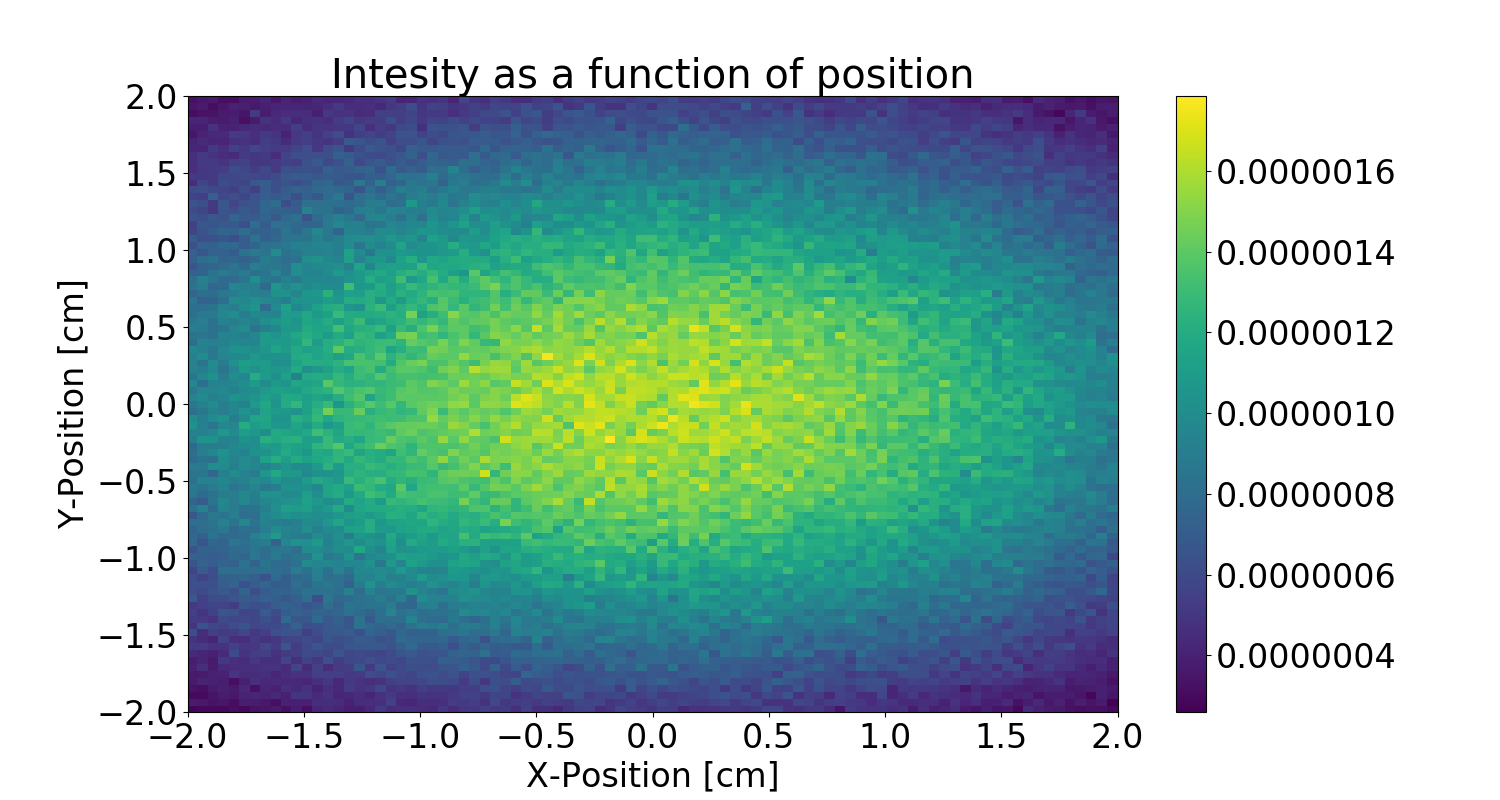
\includegraphics[width=1\textwidth]{psd_ess_simple_after.png}
\caption{Positionen af neutronerne efter den simple ESS guide}
\end{figure}


\begin{figure}[H]
\centering
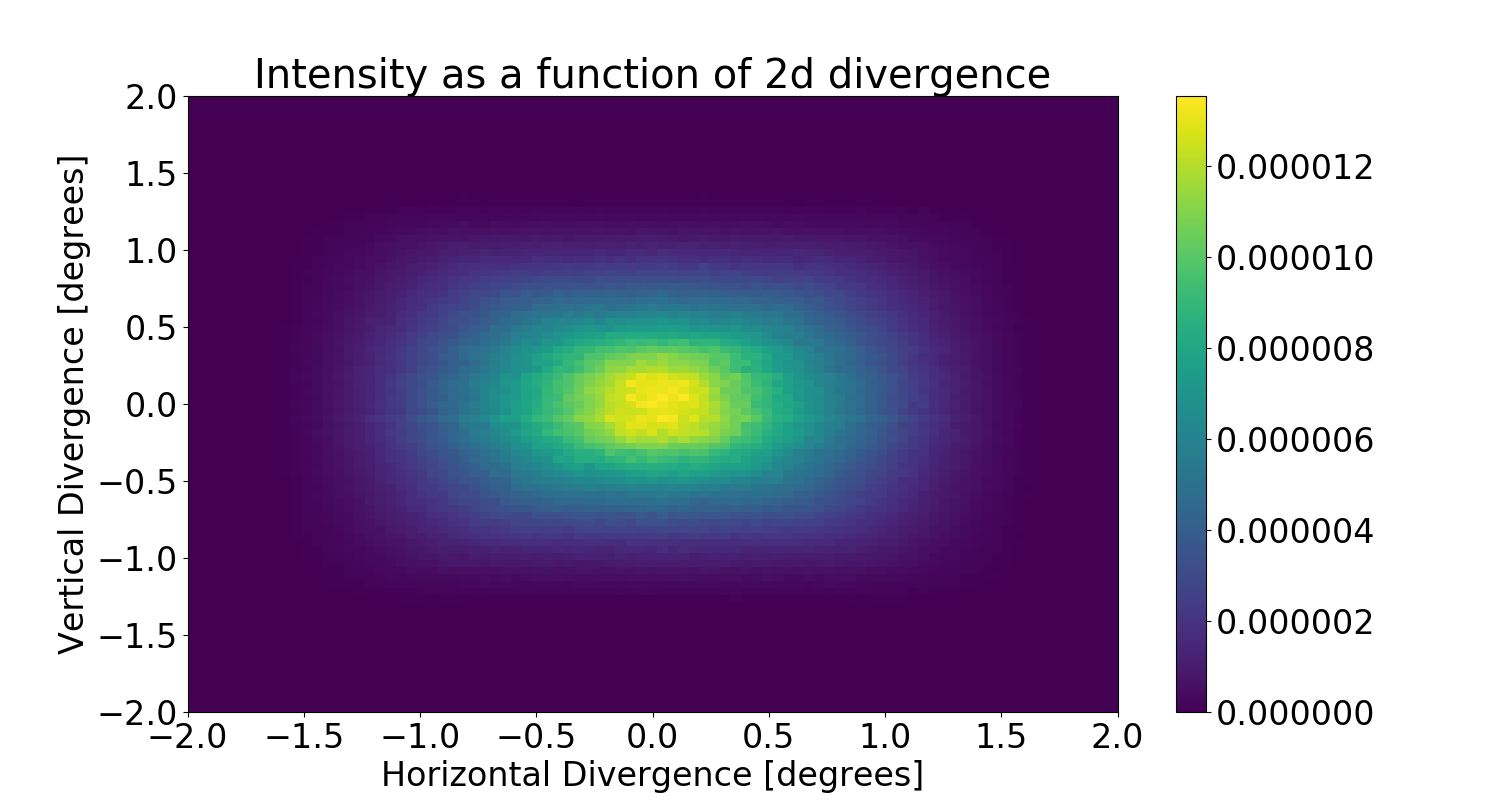
\includegraphics[width=1\textwidth]{div_ess_simple_before.png}
\caption{Divergensen inden guiden}
\end{figure}

\begin{figure}[H]
\centering
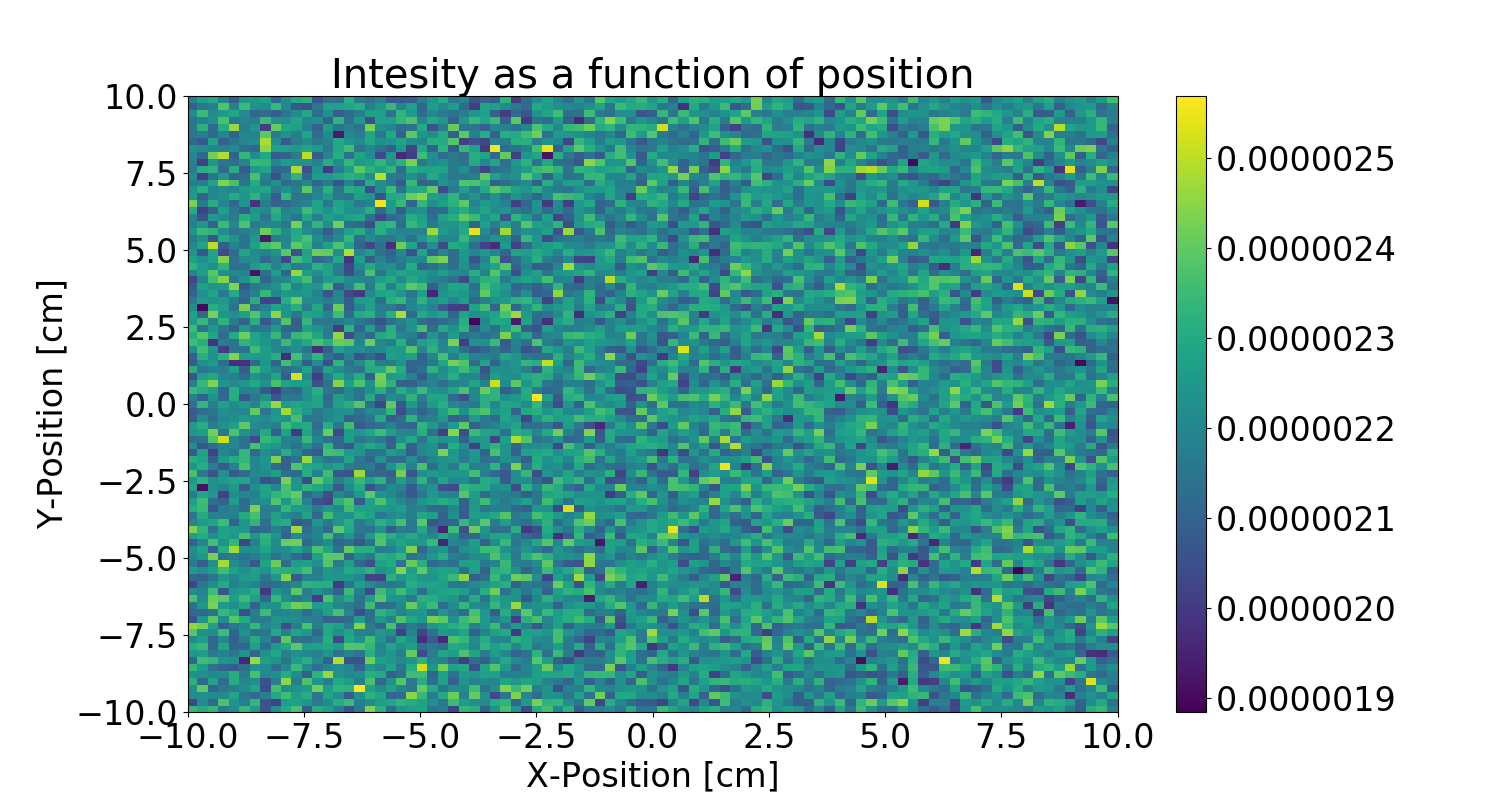
\includegraphics[width=1\textwidth]{psd_ess_simple_before.png}
\caption{Positionen af neutronerne inden guiden}
\end{figure}



\subsection{Realistisk ESS geometri}

\begin{figure}[H]
\centering
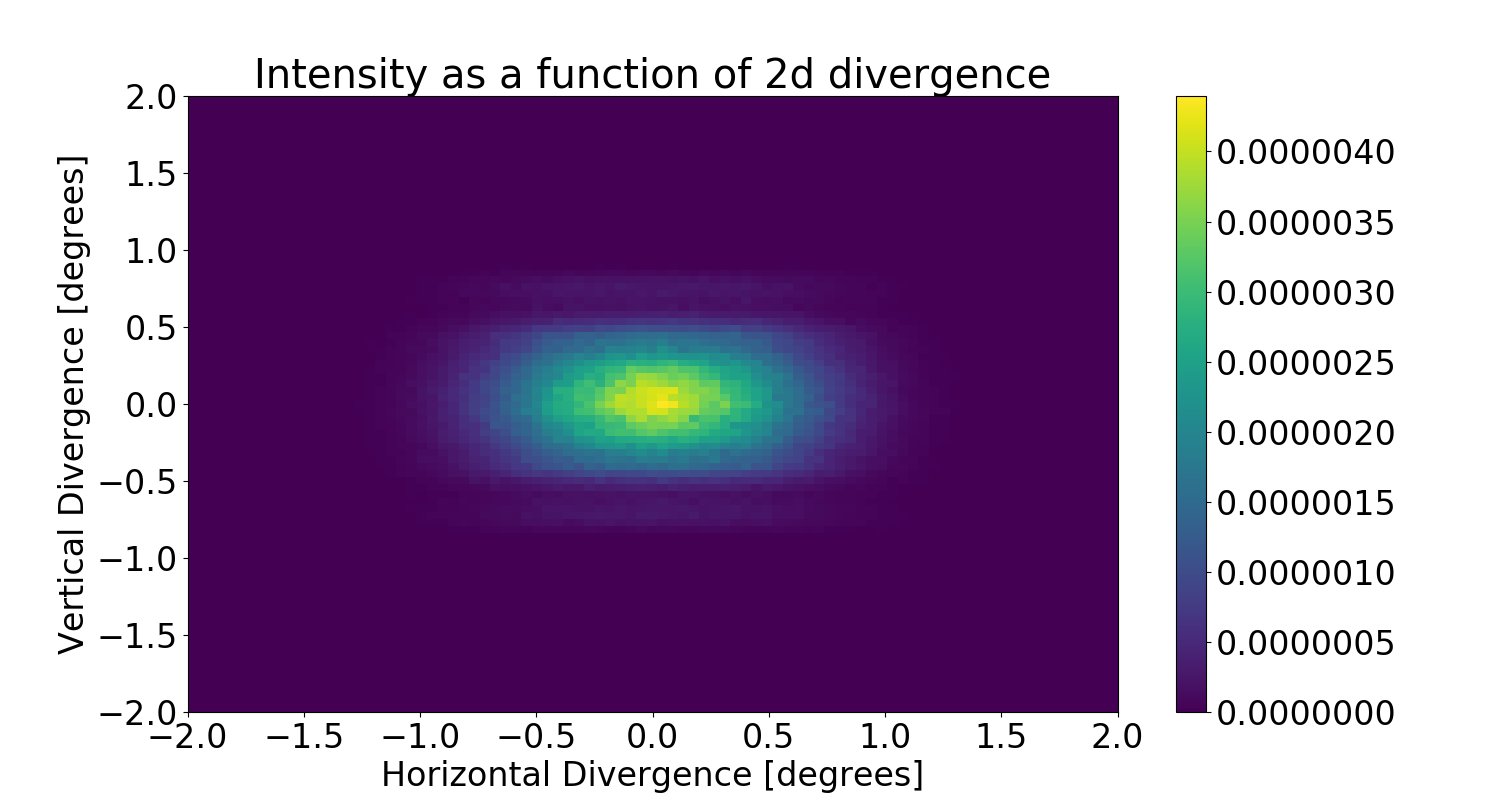
\includegraphics[width=1\textwidth]{div_after_ess_brill_optimized.png}
\caption{Divergensen ved prøven efter vores optimerede guide}
\end{figure}

\begin{figure}[H]
\centering
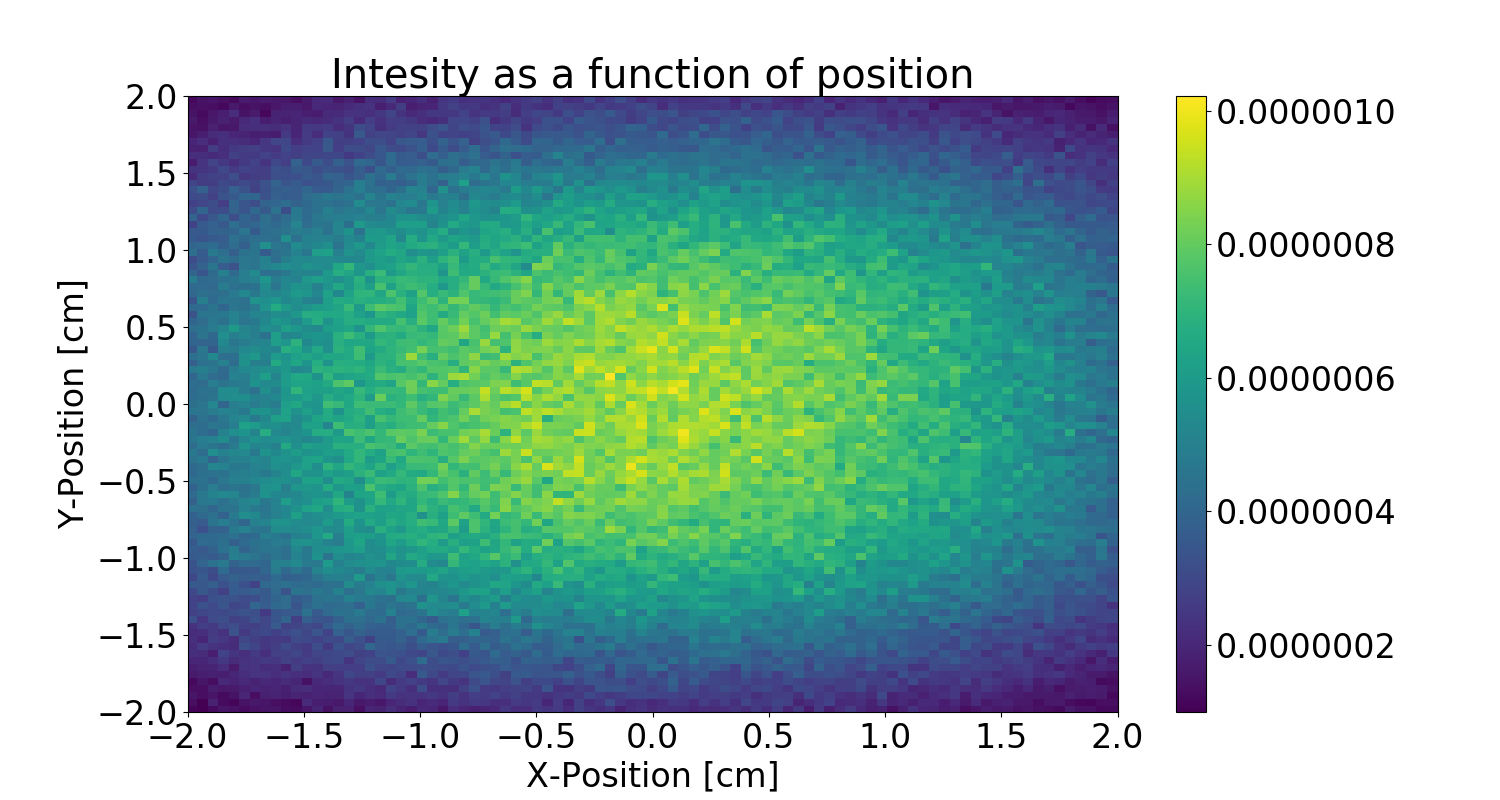
\includegraphics[width=1\textwidth]{psd_after_ess_brill_optimized.png}
\caption{Positionen af neutronerne ved prøven efter vores optimerede guide}
\end{figure}

\begin{figure}[H]
\centering
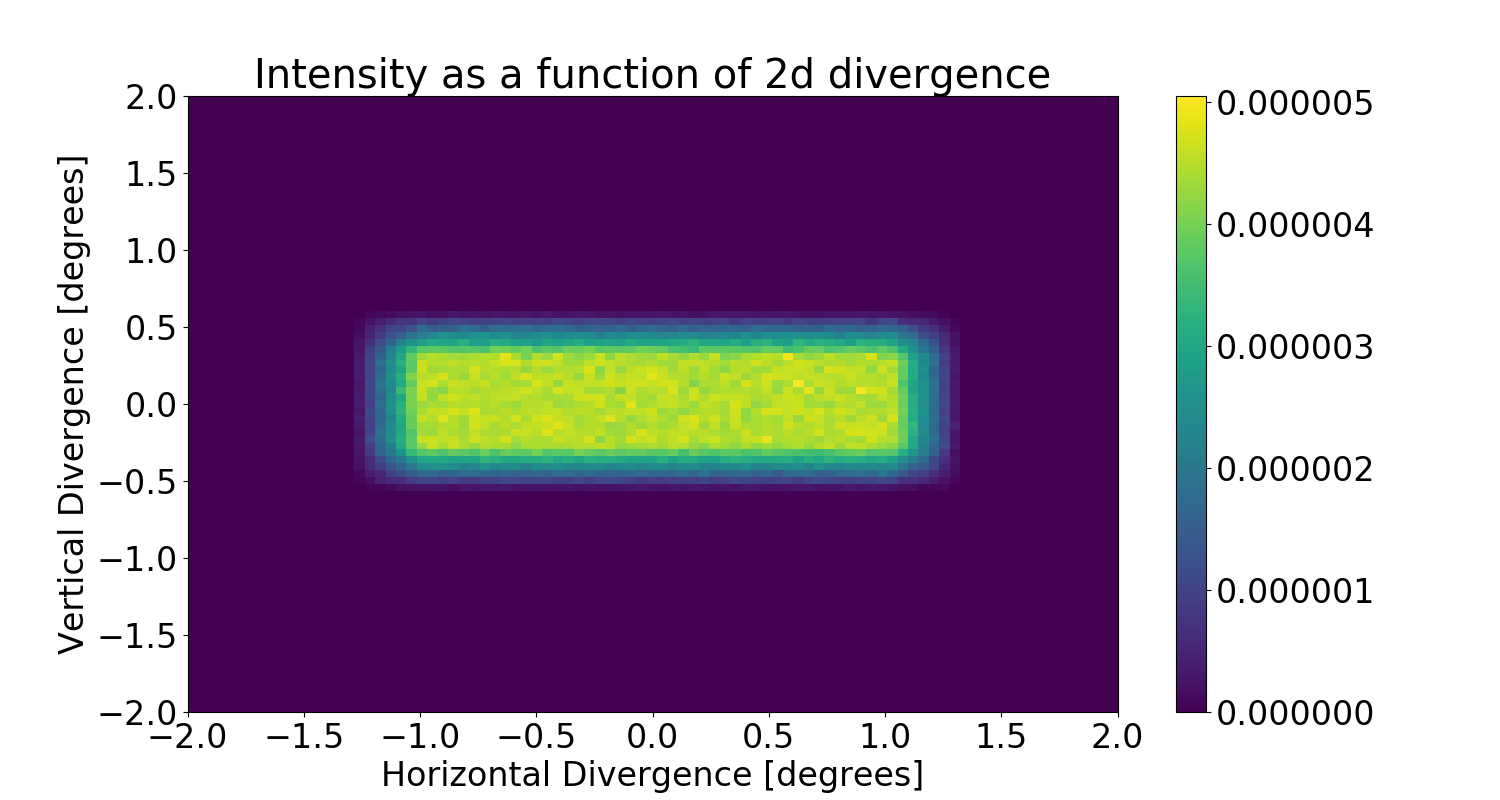
\includegraphics[width=1\textwidth]{div_before_ess_brill_optimized.png}
\caption{Divergensen ved kilden, inden vores optimerede guide}
\end{figure}

\begin{figure}[H]
\centering
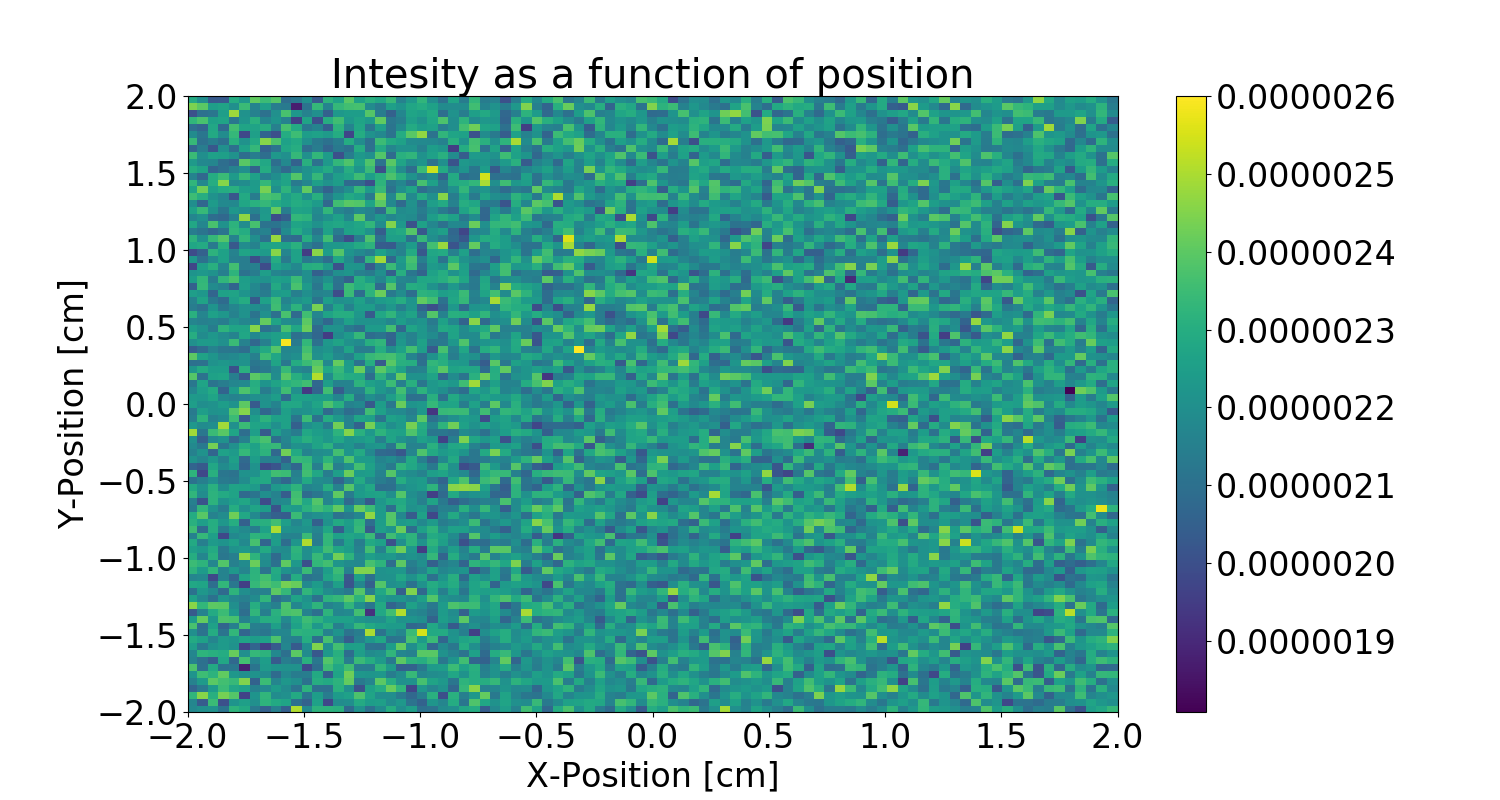
\includegraphics[width=1\textwidth]{psd_before_ess_brill_optimized.png}
\caption{Positionen af neutronerne ved kilden, inden vores optimerede guide}
\end{figure}



%% Appendix slut! %%

\end{document}

